\documentclass{article}
% if you need to pass options to natbib, use, e.g.:
%     \PassOptionsToPackage{numbers, compress}{natbib}
% before loading neurips_2023


% ready for submission
\usepackage[preprint]{neurips_2023}

% to compile a preprint version, e.g., for submission to arXiv, add add the
% [preprint] option:
%     \usepackage[preprint]{neurips_2023}


% to compile a camera-ready version, add the [final] option, e.g.:
%     \usepackage[final]{neurips_2023}


% to avoid loading the natbib package, add option nonatbib:
%    \usepackage[nonatbib]{neurips_2023}

\usepackage{amsmath}
\usepackage{graphicx}
\usepackage{caption}
\usepackage{float}
\usepackage[utf8]{inputenc} % allow utf-8 input
\usepackage[T1]{fontenc}    % use 8-bit T1 fonts
\usepackage{hyperref}       % hyperlinks
\usepackage{url}            % simple URL typesetting
\usepackage{booktabs}       % professional-quality tables
\usepackage{amsfonts}       % blackboard math symbols
\usepackage{nicefrac}       % compact symbols for 1/2, etc.
\usepackage{microtype}      % microtypography
\usepackage{xcolor}
\usepackage{cleveref}
\usepackage{enumerate}
\usepackage{listings}         % colors
\usepackage{changepage}  % For adjusting margins


\definecolor{codegreen}{rgb}{0,0.6,0}
\definecolor{codegray}{rgb}{0.5,0.5,0.5}
\definecolor{codepurple}{rgb}{0.58,0,0.82}
\definecolor{backcolour}{rgb}{0.95,0.95,0.92}

\lstdefinestyle{mystyle}{
    backgroundcolor=\color{backcolour},
    commentstyle=\color{codegreen},
    keywordstyle=\color{magenta},
    numberstyle=\tiny\color{codegray},
    stringstyle=\color{codepurple},
    basicstyle=\ttfamily\footnotesize,
    breakatwhitespace=false,
    breaklines=true,
    captionpos=b,
    keepspaces=true,
    numbers=left,
    numbersep=5pt,
    showspaces=false,
    showstringspaces=false,
    showtabs=false,
    tabsize=2
}

\lstset{style=mystyle}


\title{Machine Learning Project Report}

\author{
    Jop Zitman 2023280072\\
    Department of Computer Science\\
    Tsinghua University\\
    Beijing, China \\
    \texttt{lilw23@mails.tsinghua.edu.cn} \\
    \And
    Lauriane Teyssier 2023280008\\
    Department of Computer Science\\
    Tsinghua University\\
    Beijing, China \\
    \texttt{yell23@mails.tsinghua.edu.cn} \\
}

% Document
\begin{document}

    \maketitle

    \begin{abstract}
        The increasing sophistication and frequency of phishing attacks pose a significant threat in the digital era, highlighting the need for advanced detection methodologies.
        This study explores the application of machine learning and deep learning techniques to classify phishing URLs in the wake of an alarming escalation in cyber threats.
        Our research encompasses a comprehensive evaluation of various machine learning and deep learning models, including Logistic Regression, Support Vector Machine, Naive Bayes, Nearest Neighbors, and sophisticated neural network architectures like CNNs and LSTMs. We also delve into the realm of Large Language Models (LLMs) for phishing URL detection.

        By establishing a benchmark on a unified dataset, we aim to provide an objective comparison of different models.

        The outcomes of our research not only shed light on the efficacy of various models in phishing URL detection but also offer insights into future directions for enhancing the accuracy and efficiency of phishing detection.
    \end{abstract}

    \newpage
    \tableofcontents
    \newpage


    \section{Problem description and motivation}\label{sec:problem-description-and-motivation}
%    What’s the background of the problem?
%    Is it theory-driven, or deeply rooted in some useful application situations?
%    Is it important or necessary?
%    What impact will it bring if you finally solve it?

    The motivation for using machine learning to classify phishing URLs gains urgency against the backdrop of an alarming rise in cyber threats.
    Phishing, a deceptive practice where attackers pose as legitimate entities to harvest sensitive information, has not only intensified in sophistication but also in frequency.
    The Anti-Phishing Working Group's (APWG) report for the fourth quarter of 2022 provides a stark illustration: over 4.7 million phishing attacks were recorded in 2022, marking a year-over-year increase exceeding 150\% \cite{PhishingActivityTrendsReport}.
    The final quarter of that year alone witnessed 1,350,037 attacks, slightly up from the previous quarter's record of 1,270,883 incidents, indicating a persistent and escalating threat.
    APWG records a constant augmentation of the threat, as shown below.

    \begin{figure}[H]
        \centering
        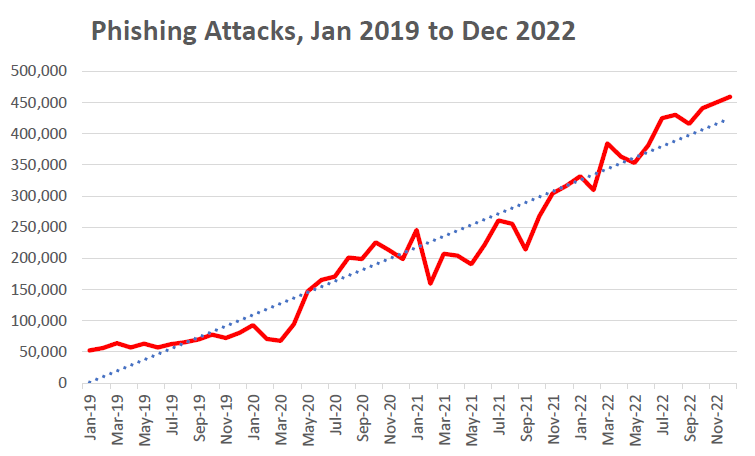
\includegraphics[width=0.8\textwidth]{report_img/shartincreasingphishing}
        \caption{Evolution of phishing from 2019 to 2022 according to APWG\cite{PhishingActivityTrendsReport}}
        \label{fig:figure}
    \end{figure}

    The financial sector had the biggest number of attacks, accounting for 27.7\% of all phishing incidents.
    Phishing attempts against webmail and software-as-a-service (SAAS) providers were also notable, comprising 17.7\% of the attacks.
    These attacks, which involve impersonating trusted parties to manipulate victims into transferring funds or revealing sensitive data, have led to losses in the billions.
    In the fourth quarter of 2022 alone, the average amount requested in wire transfer BEC attacks soared to \$132,559, marking a 41\% increase from the previous quarter.

    In addition, the FBI’s Internet Crime Complaint Center reported a near doubling of phishing incidents from 2019 to 2020.

    The methods employed in these attacks are diverse.
    The fourth quarter of 2022 saw advance fee fraud scams surpassing gift card requests as the most popular method, accounting for 39\% of all attacks.
    This shift underscores the adaptability and evolving strategies of attackers.
    Gift cards, particularly Amazon and Apple cards, remained popular among scammers, with 60\% favoring Amazon cards.

    Historically, phishing attempts were more transparent and easier to spot due to their general approach and clear warning signs.
    However, the integration of AI has led to more subtle and customized phishing strategies, using personal information to boost their believability.
    This shift calls for a detection system that is both intelligent and adaptive, capable of keeping pace with these evolving threats.

    Today's method of detecting phishing URLs mainly rely on blacklists, lists of known phishing URLs, implemented in web browsers, use Google Safe Browsing~\cite{GoogleSafeBrowsing}, or are provided by security vendors.
    However, these methods lack in speed detection for being more efficient.
    \cite{PhishingExperimentalBlackLists2009} reports after empirical analysis that less than 20\% of their phishing campaigns have been caught.
    Moreover,\cite{PhishingBlackLists} reports only 12\% overlap between two of the main phishing blacklists.

    This landscape of evolving phishing attacks underscores the critical need for fast, practical and advanced detection methods.

    The application of machine learning in phishing URL detection is one of the most promising techniques being explored.


    \section{Related works}\label{sec:related-works}

    In the realm of URL-based phishing detection, a rich literature addresses each part of the detection process, from the creation of set of databases to comparison metrics between the methodologies, including comparison of classification algorithm or data pre-processing.
    The approach can be divided into two main groups, the authors focusing on Machine Learning and and those proposing an approach based on deep learning.
    We will highlight references of both approaches.

    \subsection{Machine Learning based approaches}\label{subsec:machine-learning-based-approaches}

    \begin{itemize}

        \item An phishing URL detection method (\cite{PhishingURLDetection}) compares different Machine Learning classification algorithm.
        Their data processing involves first the detection of word statistics through 17 NLP handcrafted features, such as the brand name count, random words, or typosquatting.
        The classification is based on detecting Typosquatting and employs various algorithms like Naive Bayes, Random Forest, kNN, Adaboost, K-star, SMO, and Decision Tree.
        The study reached 97.98\% of accuracy with Weka's RFC (Random Forest Classifier).

        \item In their paper\cite{PhishSafe}, Jain and Gupta developed an anti-phishing system employing 14 handcrafted URL descriptors.
        They conducted tests using two classifiers: Naive Bayes, which achieved an accuracy of 76.87\%, and Support Vector Machine, demonstrating a higher accuracy of 91.28\%.

        \item The study presented in\cite{LexicalFeatureSelection} implemented a classification system based on lexical features extracted from URLs. Their methodology involved a feature extraction from URLs, the selection of the most relevant features through chi-square feature selection, and the utilization of various machine learning algorithms for classification.
        With nine selected features and a Random Forest (RF) classifier, they achieved their best accuracy of 98.57\%.

    \end{itemize}

    \subsection{Deep Learning based approaches}\label{subsec:deep-learning-based-approaches}

    \begin{itemize}
        \item  The Spanish national institute for security classifies in\cite{PhishingLoginURLDetection} login form URLs into malicious or legitimate categories through two distinct techniques.
        The first technique employs machine learning with text pre-processing, including symbol-based word separation, text conversion into feature vectors (use 38 features, among them the frequency of symbols, the number of digits, length, \ldots), and classification.
        Eight different classifiers have been used for comparison.
        The second technique utilizes deep learning, specifically a convolutional neural network, with no text preprocessing.
        The results show that the best performance is archived for the machine learning NLP frequency feature extraction combined with Logistic Regression (accuracy of 96.50\%).


        \item \cite{EfficientDeepLearningPhishingDetection} introduced three Deep Learning models for classifying phishing URLs, utilizing ten of the most relevant handcrafted features out of a total of 18, which included characteristics like the number of dots, length, and the presence of HTTPS. These models included Convolutional Neural Network (CNN), Deep Neural Network (DNN), and Long Short-Term Memory (LSTM). Among these, the LSTM model achieved the best performance, boasting an impressive accuracy of 99.57\%.

        \item An RCNN model to classify phishing URLs is compared with different machine learning common approaches (Naïves Bayes, Logistic Regression, random forest and XGBoost) on four different types of features (hand crafted, character embedding, character level TF-IDF and character level count vector features)\cite{CharacterLevelCNN}.
        The URL is used as input for a tokenizer and then then transformed into a matrix using one-hot encoding.
        Their RCNN model obtained 95.02\% accuracy.

    \end{itemize}

    \subsection{Large Language Models}\label{subsec:large-language-models}

    \begin{itemize}
        \item PhishBert~\cite{PhishBert} is a Bert based model that is pretrained with the manipulated token detection objective on 3 billion URLs. A classification layer is then added and fine-tuned on a smaller dataset with the objective of detecting phishing URLs. The model achieves an unspecified, but close to 100 percent accuracy depending on the amount of data in their pre-training stage.
    \end{itemize}

    \subsection{Datasets}\label{subsec:datasets}

    \begin{itemize}
        \item There exists multiple crowdsource based phasing URL collection applications. The main ones are PhishTank~\cite{PhishTank}, OpenPhish~\cite{OpenPhish}, and PhishRepo~\cite{PhishRepo}. However, due to the relatively short-lived nature of phishing sites after a phishing report, all of these do regular data cleanups. They offer a data feed that you can subscribe too, meaning that if you want to create a dataset, you have to subscribe to the feed for a while, where back-filling is not completely possible.
        \item Another popular dataset is Google SafeBrowsing\cite{GoogleSafeBrowsing}, which is integrated into several browsers. Unfortunately, they only expose a query API to check a URL for legitimacy, rather than exposing their entire dataset.
        \item JPCERT/CC is a Computer Security Incident Response Team established in Japan. The organization coordinates with network service providers, security vendors, government agencies, as well as the industry associations\cite{JPCertCC}. In 2022, they released a URL dataset of phishing sites confirmed from January 2019 to June 2022\cite{JPCertCCDataset}.
        \item Another dataset published on GitHub contains about 750k malicious URLs and 750k benign URLs\cite{VisualizingRNNInURLDetection}. The malicious set is collected by following the aforementioned PhishTank for a while. For legitimate URLs, they followed the top Alexa websites (an organization tracking most commonly visited websites).
        \item In\cite{PhishingLoginURLDetection}, it is mentioned that ``Existing URL datasets use the homepage URL from well-known websites as the legitimate. However, we think that the challenge is to determine if a login form of a website is legitimate or phishing. From our perspective, and to the best of our knowledge, publicly available datasets are not reflecting conditions that represent some real problems for phishing URL detection.'' This raises the question of whether the models built on home page-based legitimate websites are even valid (comparing apples and pears). In their dataset (PILU-90K), they only include URLs of pages which contain password fields (suggesting it's a login page).
        \item Some datasets also include further data of each URL, such as the HTML title, body, or even a screenshot. For example, the ``Phishing Websites Dataset''\cite{VisualizingRNNInURLDetection} contains the entire HTML of every URL, largely increasing the dataset size and the potential solutions of solving the problem. Such datasets are either constructed using DMOZ, CommonCrawl, or by manual fetching (using headless browsers\cite{PhishingLoginURLDetection} or simple HTTP clients). DMOZ~\cite{DMOZ} is a large human-edited web directory, which has been used in the past to create a dataset of legitimate URLs. However, this project has been discontinued in 2017, and the data is no longer maintained. CommonCrawl~\cite{CommonCrawl} is similar to DMOZ. It is a non-profit organization that crawls the web and makes the data publicly available.
    \end{itemize}


%    Different deep learning model have been used to classify websites.
%    Two main approaches occurs when trying to analyze the web: classifying a website by analyzing its content or relying on the URL to classify it
%
%    Some are directly linked
%
%    Papers detecting phishing URL for example from 2022
%    https://ieeexplore.ieee.org/document/9759382.
%    In their state of the art, the author evokes different classification machine learning algorithm:
%    - Buber et al. [25] 17 NLP (Natural Language Processing) handcrafted
%    features such as the number of sub-domains, random words,
%    digits, special characters and length measurements over the
%    URL words
%
%    StringToWordVector


    \section{Proposed method}\label{sec:proposed-method}

    \subsection{Approach}\label{subsec:approach}


%    Method chosen: offline URL classification
%    Advantages of the method chosen: fast computation, language independent
%
%    We aim to find the bests performances on classifying malicious from legitimate URL by implementing comparative machine learning and deep learning approaches.
%
%    Regarding machine learning, the modeling process consists in three steps: pre processing (converting URL into text), extraction of feature and classification.
%    We want to compare the performance of different classifiers, by optimizing simultaneously the construction of the feature and their selection.
%
%    Regarding deep learning, the performance mainly depends on the layer architecture.
%    Our objective is to try replicating one or two neurons architectures among the more performing on previous works.
%    Some additional data treatment may be done.
%
%    Very rich literature on the subject, we want to benchmark them and compare them on the same dataset.
%
%    What are the motivations for you to choose it?
%    Which datasets do you propose to
%    experiment on?
%    What baseline approaches do you plan to compare with?
%    How do you implement your proposed method based on the dataset?
%    It is ok to change and improve it later but now try to describe it as detailed as possible.
%
%    Inspired from different techniques and analysis used to classify URL, we will try to identify the category of website the URL relates to
%
%    - test of different ML algorithm for performance comparison (linear regression, deep neural network, modification of pre train text analysis model) to compare and select the best model
%
%    - test of different datasets, and the results of training on one/test on the other (different datasets available on kaggle and on the net) - possibility on comparing the results depending on the date/epoque of the dataset, the countries they are from, \ldots and see what comes up
%
%    - what do the domain name tells us about the website?
%    do we have some better performances analyzing some complete URL? If yes, how much does it increases the performance of the model?
%
%    - Different approaches : making clusters with imposing the categories that we expect, or seeing what categories it makes on its own, by clustering and finding out what each clusters is linked with

    We want a fast approach to classify URL instantly, that could be integrated within navigator to complete blacklists.
    To achieve time efficiency, we want to only rely on the URL, not on the content of the page or any content that would need to send a request to the website.
    Therefore, we chose to classify phishing websites relying on their URL only.
    Strikingly, many of the existing studies on phishing URL detection are each based on different datasets and methodologies, each displaying a higher accuracy than the previous one.
    However, we were intrigued by the different results that studies have on same models (for example machine learning models) on similar datasets.
    From all these studies, it seemed difficult to establish any ranking or argument comparison of the different models, since each one had the best results on its new introduced approach.
    For this reason, we chose to establish a benchmark of the different solutions.
    By implementing them on the same dataset, relying on the different studies from the literature, we aim to establish a more objective classification.
    In addition, this process allows us as a students to develop our critical sense of studies (learn to detect what can be improved from a study, from what is strong argumentation).

    Similar to the existing studies, we will create hand-crafted features from the URL and perform feature selection to reduce the dimensionality of the data.

    We explored the following models:
    \begin{figure}[H]
        \centering
        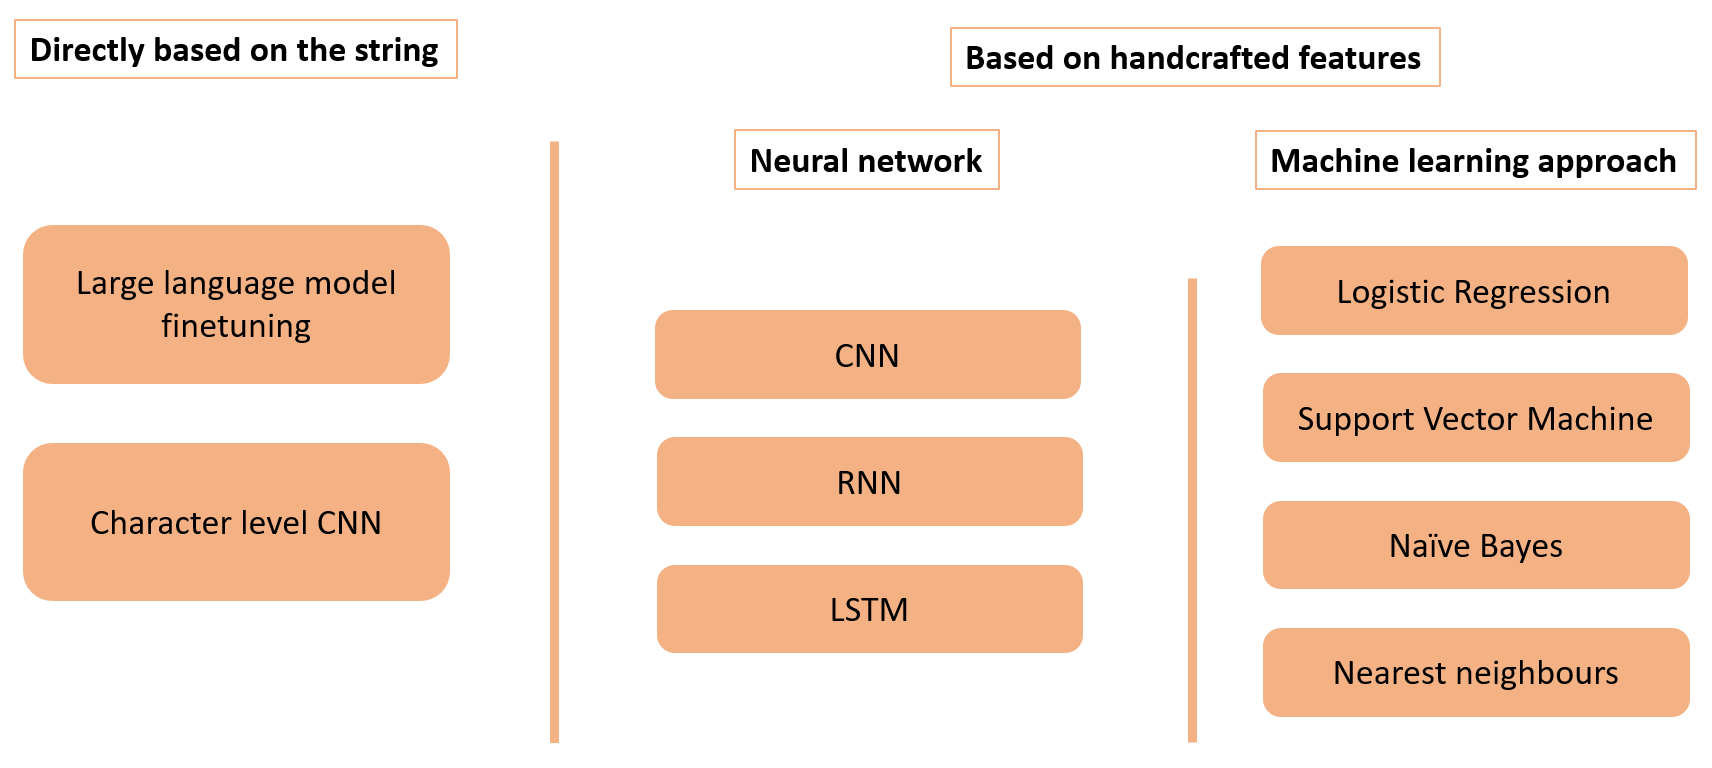
\includegraphics[width=\linewidth]{report_img/modelspresentation}
        \caption{Overview of the different models implemented}
        \label{fig:model_presentation}
    \end{figure}

    \subsection{Dataset}\label{subsec:dataset}

    In our initial project proposal, we intended to utilize the PILU-90K~\cite{PhishingURLDetection}, because being large and recent.
    However, accessing this dataset proved to be challenging due to the requirement of a formal request by a professor supervising the project.
    Consequently, we shifted our focus to the most extensive dataset identified in our research, specifically the one proposed in~\cite{VisualizingRNNInURLDetection}.
    Among the available datasets with sufficient volume for neural network model training, this particular dataset is the most recent and provides open access.
    The age of the dataset was a crucial criteria:\cite{PhishingLoginURLDetection} report up to 10\% decrease of accuracy by using 5 years old training data.

    Originally, this dataset is tailored for training Neural Network models, with its data already encoded in integer array formats.
    To adapt this dataset for broader Machine Learning applications, we undertook a preprocessing step to convert these integer arrays back into textual URL formats.
    Furthermore, in our exploration of neural network methodologies, we are not only utilizing the original vectorization techniques of the dataset but also experimenting with alternative vectorization strategies.

    We've thought about manually generating datasets, in case we are unable to find public datasets.
    For instance, we could extract malicious URLs from phishing e-mail datasets.
    We could also manually gather URLs from PhishTank, OpenPhish, or PhishRepo, but we expect that the few weeks that we may be able to gather URLs will not give us a large enough dataset, also considering the need for verification and the unknown project grade contribution of dataset generation.

    In addition, if we want to follow the methodology described in ~\cite{PhishingLoginURLDetection}, we would have to manually crawl hundreds of thousands of web pages using headless browsers in order to find the login page.
    We did not consider this option because of the time and resources required, especially since browsers take many resources and are hard to parallelize.
    We also expected issues with running into Web Application Firewalls when visiting so many websites, further decreasing the quality of our dataset.

    \subsubsection{Preprocessing}\label{subsubsec:preprocessing}
    Since the original dataset is already encoded in a character embedding integer array format, and we want to create our own feature vector, we need to convert the dataset back to a textual URL format.
    In the directory \texttt{data\textbackslash convert}, we provide a script \texttt{dill\_to\_csv.py} to convert the dill dataset from the integer array format to a textual URL format.

    We provide another script \texttt{csv\_to\_feature\_vector.py} which converts this csv from textual URL format to a feature vector using the feature selection described in \Cref{subsec:establishement-of-the-feature-vector}.

    \subsection{Machine Learning Frameworks}
    For the machine learning framework, we decided to use RAPIDS AI’s cuML as opposed to sklearn due to its significant performance advantages when dealing with large datasets.
    Leveraging the GPU, cuML achieves a 10 to 50 times speedup compared to CPU-bound libraries like sklearn.
    Unlike sklearn, which operates primarily on CPUs and can struggle with scalability, cuML is designed to handle vast amounts of data more efficiently.
    Additionally, its API mirrors that of sklearn, offering ease of use and a familiar environment for those accustomed to sklearn, but with the added benefit of GPU acceleration.
    This makes cuML an attractive choice for projects without the need for extensive adjustment to new programming paradigms.

    The framework does not provide solutions to perform hyperparameter optimization, so we picked another library called hyperopt for this.
    Hyperopt is a powerful and versatile library for hyperparameter optimization in machine learning algorithms.
    Hyperopt employs Bayesian optimization, specifically the Tree of Parzen Estimators (TPE) algorithm, which stands out for its efficiency in navigating the hyperparameter space.
    Unlike the exhaustive search approach used in sklearn's GridSearchCV or the randomness of RandomizedSearchCV, Hyperopt's method is more focused and informed, learning from each iteration to concentrate on the most promising hyperparameter combinations.
    Optuna is another library that offers similar features.
    Hyperopt was a more appropriate choice for this project due to our experience with it and its ability to serve all our hyperparameter needs.

    Considering that most of the tested Machine Learning algorithms require little memory, we tried to use hyperopt's \texttt{MongoTrials} to parallelize the parameter search.
    We saw however that it led to no speedup, as the process was mainly GPU processing bound rather than memory bound.

    \subsection{Deep Learning Frameworks}
    For the deep learning framework, we decided to use Keras due to its simplicity and ease of use.
    Although Keras is known for integrating with TensorFLow, the new Keras 3.0 API also supports other backends.
    Throughout the project, we switched backends multiple times, but we ultimately settled on using PyTorch.
    Using the dedicated GPU in our laptops, the PyTorch backend had the most predictable performance and memory and was the easiest to debug.
    By using such a high level framework, we were able to quickly iterate on different architectures and hyperparameters, rather than focusing on the implementation details of the neural networks.
    For instance, Keras provides simple callbacks to save the best model, and to stop training early if the validation loss does not improve for a certain number of epochs.
    It also provides built-in metric functions, such as accuracy, precision, recall, and F1 score.


    \section{ML models based on handcrafted features}\label{sec:models-based-on-handcrafted-features}

    Considering approaches that rely on handcrafted features is crucial, especially when we want to use ML techniques, not only neural networks.
    Creating handcrafted features enables us to reduce the dimension of the data, so to have a faster treatment and analysis afterwards.
    Intuitively, the information contained by an URL could be encoded into a far smaller dimension compared to simply having a dimension for each character or word.
    Humans are able to understand the meaning of an URL by recognizing certain features, such as the presence of a brand name or the words in the path.
    For this project, we will try to find such meaningful features.
    In addition, we will attempt to select the best number of features, so that we can reduce the dimensionality of the data as much as possible, while still achieving good results.

    On the other hand, it is important to note that handcrafted features require human interpretation of the URL, which is bad in general because it introduces biases or lost of information that a machine learning algorithm could have found.

    \subsection{Establishment of the feature vector}\label{subsec:establishement-of-the-feature-vector}

    For this project, we have picked several features based on existing research, and added several new features that we thought would be useful.
    We have left out features that require complex language processing.
    Some features may overlap others, so may contribute less to the information gain, so we will try to discover which of the selected features are the most important.
    This way we can narrow down the feature vector to the most important features for detecting phishing URLs, which will reduce the dimensionality of the data and speed up the training process.

    \subsubsection{Computations of different features}

    \begin{table}[H]
        \begin{adjustwidth}{-3cm}{}
            \centering
            \begin{tabular}{|c|p{4cm}|p{5cm}|c|c|c|c|}
                \hline
                \textbf{No.} & \textbf{Feature Name}           & \textbf{Feature Description}                   & \textbf{Chi Score} & \textbf{Chi Ranking} & \textbf{Info Gain Score} & \textbf{Source} \\ \hline
                1            & Number of Dots                  & Number of `.' in the URL                       & 64216.34           & 7                    & 0.0944                   & ~\cite{LexicalFeatureSelection}             \\ \hline
                2            & Number of Hyphens               & Number of `-' in the URL                       & 517655.65          & 1                    & 0.0747                   & ~ ~\cite{PhishSafe,LexicalFeatureSelection} \\ \hline
                3            & Number of @                     & Number of `@' in the URL                       & 4465.27            & 14                   & 0.0022                   & ~\cite{PhishSafe,LexicalFeatureSelection} ~ \\ \hline
                4            & Number of ?                     & Number of `?' in the URL                       & 9006.72            & 11                   & 0.0129                   & ~\cite{LexicalFeatureSelection}             \\ \hline
                5            & URL Length                      & Length of the URL                              & 291038.97          & 6                    & 0.0283                   & ~\cite{PhishSafe,LexicalFeatureSelection}   \\ \hline
                6            & Number of Digits                & Number of digits in the URL                    & 312225.09          & 5                    & 0.1280                   & ~\cite{PhishingLoginURLDetection}           \\ \hline
                7            & Number of /                     & Number of `/' in the URL                       & 25682.89           & 8                    & 0.0621                   & ~\cite{LexicalFeatureSelection}             \\ \hline
                8            & Number of //                    & Number of `//' in the URL                      & 194.38             & 16                   & 0.1334                   & ~\cite{PhishSafe,LexicalFeatureSelection}   \\ \hline
                9            & Use of HTTPS                    & Counts occurrences of `https'                  & 164109.06          & 4                    & 0.1229                   & ~\cite{PhishSafe}                           \\ \hline
                10           & Use of HTTP                     & Counts occurrences of `http'                   & 215.22             & 15                   & 0.1470                   & ~\cite{PhishSafe,LexicalFeatureSelection}   \\ \hline
                11           & Use of WWW                      & Counts occurrences of `www'                    & 1150.42            & 13                   & 0.0482                   & ~\cite{PhishingURLDetection}                \\ \hline
                12           & IP Address Usage                & 1 if IP address is used, 0 otherwise           & 19994.97           & 9                    & 0.0113                   & ~\cite{LexicalFeatureSelection}             \\ \hline
                13           & Suspicious Word Count           & Counts suspicious words in the URL             & 517281.65          & 2                    & 0.1526                   & ~\cite{PhishSafe,LexicalFeatureSelection}   \\ \hline
                14           & Gift Card Suspicious Word Count & Counts gift card suspicious words in the URL   & 20.61              & 26                   & 0.0                      & new feature \\ \hline
                15           & TLD Position                    & Position of Top-Level Domain in URL            & 19567.30           & 10                   & 0.0410                   & ~\cite{PhishSafe}                           \\ \hline
                16           & Path Length Ratio               & Ratio of path length to URL length             & 65.01              & 20                   & 0.0246                   & ~\cite{LexicalFeatureSelection}             \\ \hline
                17           & Suspicious Char Count           & Counts suspicious characters in URL            & 96221.30           & 7                    & 0.0510                   & ~\cite{LexicalFeatureSelection}             \\ \hline
                18           & Symbol as Last Char             & 1 if last character is a symbol, 0 otherwise   & 0.00               & 21                   & 8.97e-05                 & ~\cite{LexicalFeatureSelection} \\ \hline
                19           & Redirection Count               & Counts number of `.' in subdomain              & 263490.59          & 12                   & 0.0400                   &                                             \\ \hline
                20           & IP Address Presence             & 1 if IP address present, 0 otherwise           & 19861.37           & 17                   & 0.0102                   & ~\cite{PhishSafe,LexicalFeatureSelection}   \\ \hline
                21           & Subdomain Count                 & Number of subdomains                           & 67213.42           & 14                   & 0.1247                   & ~\cite{PhishSafe}                           \\ \hline
                22           & Port Presence                   & 1 if port number present, 0 otherwise          & 387.36             & 18                   & 0.0                      & ~\cite{LexicalFeatureSelection}             \\ \hline
                23           & Unicode Char Count              & Number of unicode characters                   & 290705.11          & 6                    & 0.0279                   & ~\cite{LexicalFeatureSelection}             \\ \hline
                24           & Query Presence                  & 1 if query present in the URL, 0 otherwise     & 0.00               & 22                   & 0.0                      & ~\cite{LexicalFeatureSelection}             \\ \hline
                25           & Special Char Ratio              & Ratio of special characters to URL length      & 559.19             & 25                   & 0.0867                   & \cite{PhishingLoginURLDetection} \\ \hline
                26           & Misspelled Word Presence        & 1 if misspelled words are present, 0 otherwise & 9199.83 & 24 & 0.1170 & new feature \\ \hline
            \end{tabular}
            \caption{Summary of Features Implemented for Phishing URL Detection}
            \label{tab:features}
        \end{adjustwidth}
    \end{table}

    As mentioned before, some features have been designed by ourselves after reading on phishing.
    For example, we have added a feature that counts the number of times gift card related words appear in the URL.
    We believe this feature is important because gift cards are a common target of phishing attacks~\cite{PhishingActivityTrendsReport}.
    In our dataset, 200 URLs contained such words.
    We also added a feature that checks whether the URL contains misspelling by using the Python package fuzzywuzzy, which uses Levenshtein distance to measure the similarity between two strings.
    We compare words in the URL to a list of words that are commonly misspelled in phishing URLs (such as \texttt{Google} or \texttt{mastercard}).

    Some of the features proposed in~\cite{PhishSafe} require additional lookups to external sources.
    Due to limited resources, we decided to not include these features in our feature vector.
    In addition, such the need to querie such external sources may make it more unlikely to be implemented in a browser extension.
    \begin{itemize}
        \item DNS lookup: there may be a pattern in the A/CNAME/NS/MX records of phishing URLs.
        \item URL not matching WHOIS records: If the domain name of suspicious web page is not matched with the WHOIS database record, then the web page may be considered as phishing.
        \item Age of Domain: If the age of website is less than 6 month, then chances of fake web page are more from.
    \end{itemize}

    \subsubsection{Most important features}

    We expect that some features will be more important than others, and that some features overlap others.
    To improve our method in terms of computation speed as well as interpretability, we want to keep only the most relevant features.
    As provided in\cite{LexicalFeatureSelection}, we expect only a small number of features to be improve the accuracy.
    As showed on their graph below, above a threshold, the accuracy of their model do not increase anymore with the number of features used.

    \begin{figure}[H]
        \centering
        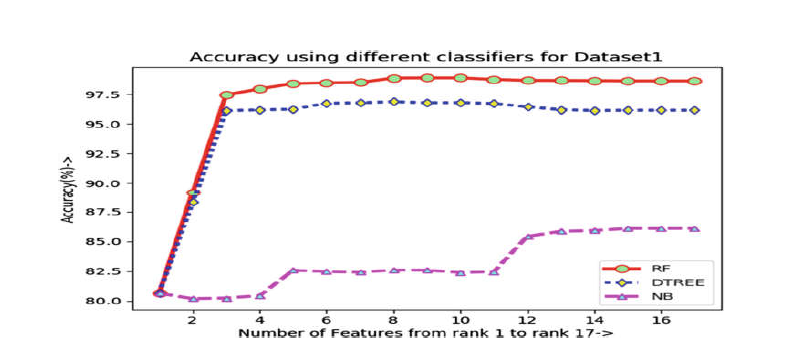
\includegraphics[width=\textwidth]{report_img/lexicalfeatureselectionaccuracygraph}
        \caption{Feature wise accuracy of classifiers from\cite{LexicalFeatureSelection}}
        \label{fig:kEvolution}
    \end{figure}

    We commonly encountered the following methods to reduce the dimensionality of the data and in the context of feature selection for binary classification of phishing URLs, we examined the advantages and disadvantages of these methods:
    \begin{itemize}
        \item \textbf{Principal Component Analysis (PCA)}: can reduce the dimensionality of the data, but instead of selecting relevant features, it transforms the data into a new space. We loose the interpretability of the features, which is the main motive behind handcrafted features. In addition, the encoding of a new URL for testing it is more complex, compared to feature selection. Therefore, we loose the practicality of the approach. This solution is more interesting for high dimensional data, and data where the different meanings of the features do not matter.
        \item \textbf{Singular Value Decomposition (SVD)}: same as PCA, it transforms the data into a new space, and we loose the interpretability of the features.
        \item \textbf{Variance Thresholding}: this method is interesting when we have a lot of features, and we want to keep only the features that have a variance above a certain threshold. However, we have two types of features: binary, and counts. Even if we normalize all features between zero and one, the variance is influenced by the nature of the feature. Therefore, we cannot compare the variance of the different features, and we cannot use this method.
        \item \textbf{Information Gain}: as demonstrated in\cite{EfficientDeepLearningPhishingDetection} for feeding into neural networks, this method excels in measuring entropy reduction, and is effective with both categorical and continuous variables. However, it falls short in capturing the correlation between features since it assesses them in isolation.
        \item \textbf{Chi-Square}: used in\cite{LexicalFeatureSelection}, this method quantifies the independence, or lack thereof, between categorical variables and the target variable, offering a straightforward and computationally efficient approach for binary classification. It is also known for its effectiveness in assessing the relevance of categorical features in classification tasks.
    \end{itemize}

    Chi-square score is computed using the observed and expected frequencies of the features following the formula:
    \begin{equation}
        \chi^2 = \sum \frac{(O_i - E_i)^2}{E_i}\label{eq:equation}
    \end{equation}
    where \( \chi^2 \) is the Chi-Square statistic, \( O_i \) is the observed frequency, and \( E_i \) is the expected frequency under the null hypothesis that the feature and the target are independent.

    Considering these factors, Chi-Square emerged as the most appropriate technique for our study.
    Its simplicity, efficiency, and focus on categorical feature relevance align well with the nature of our dataset and the objectives of our phishing URL classification project.
    For experimental reasons and comparison purposes, we also tried to use Information Gain.

    \Cref{fig:k_search_logistic_regression} shows the influence of the number of features k on the accuracy of the logistic regression.
    We use the default hyperparameters of the logistic regression, as we're not specifically concerned with the performance of this model, but rather with the effect of the number of features on the performance of the model.

    \begin{figure}[H]
        \centering
        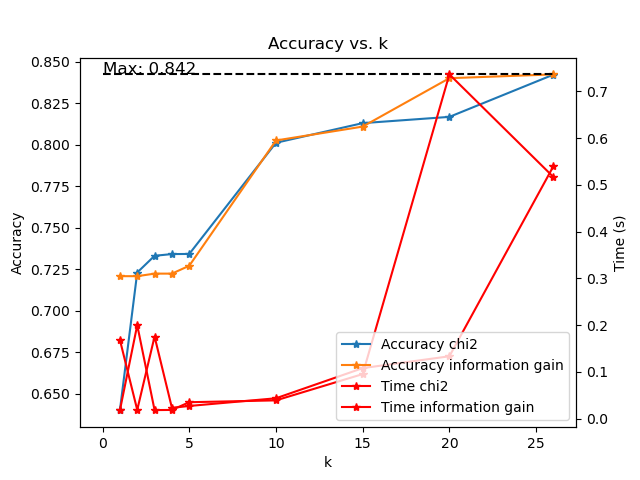
\includegraphics[width=0.8\textwidth]{report_img/k_search/logistic_regression}
        \caption{Influence of number of features k on logisitic regression accuracy and computing time. Selected using chi square or information gain.}
        \label{fig:k_search_logistic_regression}
    \end{figure}

    Compared to \Cref{fig:kEvolution}, our graph do not show a very flat line with parameters nearly not influencing the model after a certain number.
    The evolution shows a plateau, indicating that the firsts selected features may be redundant.
    A method taking into account interactions between features would be even more suited for an efficient feature selection.

    By plotting Information Gain as well, we wanted to confirm experimentally the choice of chi square as a selection method.
    We observed that both methods have similar performances except for Naive Bayes were Information Gain outperforms Chi square, and for Random Forest where Chi square significantly outperforms (\Cref{sec:appendixA}).

    The accuracy constantly increases showing that combination of parameters bears meaning and helps the model improving even with the last features.
    By looking at the graphs plotted in \Cref{sec:appendixA}, we observed that each model has a different behavior towards the features.
    Moreover, the computing time associated to using the full feature vector for computing results or fitting the model compared to a reduced version of it is not significant.
    Therefore, for the rest of this project, we chose to work with the full feature vector of 26 features.

    \subsubsection{Implementation}\label{subsubsec:implementation}

    \subsection{Motivation between the choices of the different machine learning models}\label{subsec:motivation-between-the-choices-of-the-different-machine-learning-models2}

    We have chosen various statistical methods to address our binary classification problem, encompassing both linear and non-linear models.
    Our selection of these models was influenced by existing research as we aimed to replicate them and conduct a thorough cross-sectional comparison.
    Additionally, we aimed to ensure a comprehensive representation of different model types to gain a well-rounded perspective on various approaches and their performances.
    We thoroughly describe the strengths and weaknesses of each model, allowing us to gain a deep understanding of our results and provide readers with a clear comprehension of the different models and their relevance to our problem.

    \subsubsection{Logistic Regression}
    To establish a baseline for comparing the performance of our other models, we decided to implement a simple model.
    Its simplicity allows for practical experimentation and ensures that the results are easily interpretable.

    \subsubsection{Support Vector Machine}\label{subsubsec:support-vector-machine}
    The reason behind selecting the Support Vector Machine (SVM) was to use a non-linear kernel and obtain non-linear decision boundaries through the kernel trick.
    However, due to optimization constraints, we had to settle for a linear kernel as it proved to be the fastest for training on our dataset, and it was the only available method when using cuML.
    As a result, we expect a similar outcome to logistic regression, but we still trained this model to confirm our reasoning.

    \subsubsection{Naives Bayes}
    Naive Bayes is a linear classifier as well, relying on the assumption of independence between the features.
    Even though we try to select only relevant features through our feature selection process, we still expect some correlation between the features.
    Therefore, we expect this model to perform worse than the previous ones.
    In addition, empirical studies like\cite{MLmodelsComparison} shows that this model in general performs worse than other models.
    However, it may still be interesting to verify this hypothesis, comparing our results with the other models and some of the studies that uses it.

    On another note, considering that the performance of this model relies so heavily on the feature independence, we tested its relevance as a feature selector.
    Unfortunately, as precised in~\cite{NaiveBayesBackground}, `the strength of feature dependencies (i.e. the class-conditional mutual information between the features) ’ignored’ by naive Bayes is not a good predictor of its classification error`.
    Therefore, the results on this classification do not enable us to measure efficiently the efficiency of our feature selection, like we would have wished.
    A better indicator for the performance of the Naive Bayes, as proposed in\cite{NaiveBayesBackground}, would be to use the information gain, which would be less efficient than the chi square, as explained earlier.

    \subsubsection{Nearest neighbours}

    Motivation of this implementation is to have a first simple model that provides non linear decision boundaries.
    Performance of this model really relies on how good the initialization is.
    However, we can ask Python in built library to work on trying to find this best initialization.
    Interesting with this model is also the interpretability that it could provide for further studies.

    \subsubsection{Random Forest}
    Random Forest is a classifier that operates effectively with non-linear data.
    According to\cite{MLmodelsComparison}, it generally stands out when compared to similar non-linear classifiers in terms of performance and delivers robust results.
    Motivation for choosing this method is its performance, together with the understanding of the importance of features that it can provide for further interpretability.
    Additionally, it can efficiently be trained in parallel, making it well-suited for handling large datasets and particularly interesting for our configuration.

    \subsection{Results}\label{subsec:results}

    \begin{table}[H]
        \centering
        \begin{tabular}{|l|p{8cm}|l|}
            \hline
            \textbf{Model}      & \textbf{Best Hyperparameters}                                                                                                                     & \textbf{Accuracy} \\ \hline
            Logistic Regression & c: 70.2468, class\_weight: 1, fit\_intercept: 0, l1\_ratio: 0.8765, penalty: 0 & 84.24\% \\ \hline
            Linear SVC          & c: 0.0010, change\_tol: 0.0006, class\_weight: 1, fit\_intercept: 0, grad\_tol: 0.0005, loss: 1, penalized\_intercept: 0, penalty: 1, tol: 11.882 & 84.17\% \\ \hline
            Naive Bayes         & alpha: 1.1583, fit\_prior: 0                                                                                                                      & 71.53\%           \\ \hline
            Nearest Neighbors   & metric: 13, n\_neighbors: 1                                                                                                                       & 94.79\%           \\ \hline
        \end{tabular}
        \caption{Comparison of Machine Learning Models for Phishing URL Detection}
        \label{tab:model_comparison}
    \end{table}

    Choice have been made to rely on accuracy for measuring the performance of our different models because the most important for us is to

    Comparison of our results with the literature
    \begin{table}[ht]
        \centering
        \resizebox{\textwidth}{!}{
            \begin{tabular}{|l|l|l|l|l|l|l|}
                \hline
                \textbf{Study}                   & \textbf{Dataset size}          & \textbf{Random Forest} & \textbf{Naive Bayes} & \textbf{SVM} & \textbf{kNN} & \textbf{Logistic Regression} \\ \hline
                \cite{LexicalFeatureSelection}   & 276640 URL                     & 98.57                  & 82.46                & 93.21        & -            & -                            \\ \hline
                \cite{PhishSafe}                 & 10,000 URLs                    & -                      & 64.74                & 76.04        & -            & -                            \\ \hline
                \cite{PhishSafe}                 & 25,000 URLs                    & -                      & 76.87                & 91.28        & -            & -                            \\ \hline
                \cite{PhishingURLDetection}      & 36,400 legit / 37,175 phishing & 97.98                  & 95.98                & -            & 95.86        & -                            \\ \hline
                \cite{PhishingLoginURLDetection} & 60k legit URL, 30k phishing    & 94.42                  & 87.72                & 93.59        & 93.18 & 92.33 \\ \hline
                \textbf{Our Study}               & 150k URL                       & 73.69                  & 71.53                & 84.17        & 94.79        & 73.69                        \\ \hline
            \end{tabular}
        }
        \caption{Comparison of Phishing URL Detection Models}
        \label{tab:model_comparison}
    \end{table}

    Our results are in the range of the studies, except for Random Forest.
    This could be related to a suboptimal parameter tuning, that is time consuming due to the high number of parameters.
    Due to our computing limitations, we decided to stop with this results.
    This could also be related to several other reasons, like our higher number of features or our different choice of library.
    We achieve our best results with kNearest Neighbours and a score of 94.79\%.

%    \cite{LexicalFeatureSelection} Using Random Forest on Lexical features of URL 276640 98.57, Precision 97.63%
%    \cite{LexicalFeatureSelection} Using Naive Bayes on Lexical features of URL 276640 82.46
%    \cite{LexicalFeatureSelection} Using SVM on Lexical features of URL 276640 93.21
%    \cite[]{PhishSafe} on 10 000 URL Naive Bayes 64.74
%    \cite[]{PhishSafe} on 10 000 URL SVM 76.04
%    \cite[]{PhishSafe} on 25 000 URL Naives Bayes 76.87
%    \cite[]{PhishSafe} on 25 000 URL SVM 91.28
%    \cite{NLPPhishingURLDetection} Random Forest 97.2 using additional NLP and wordtovec techniques to reach 278 features vector, dataset:73,575 URLs including 37,175 malicious URLs and 36,400 legal URLs.
%    \cite{NLPPhishingURLDetection} Naïve Bayes 75.5 using additional NLP and wordtovec techniques to reach 278 features vector, dataset: 73,575 URLs including 37,175 malicious URLs and 36,400 legal URLs.
%    \cite{PhishingURLDetection} datasets:36,400 legitimate URLs and 37,175 phishing URLs kNN 95.86\% on ML features
%    \cite{PhishingURLDetection} datasets:36,400 legitimate URLs and 37,175 phishing URLs Random forest 97.98\%
%    \cite{PhishingURLDetection} datasets:36,400 legitimate URLs and 37,175 phishing URLs Naive Bayes 95.98 \%
%    \cite{PhishingLoginURLDetection} dataset 60k legit, 30k phishing random forest 94.42
%    \cite{PhishingLoginURLDetection} dataset 60k legit, 30k phishing kNN 93.18
%    \cite{PhishingLoginURLDetection} dataset 60k legit, 30k phishing Naive Bayes 87.72
%    \cite{PhishingLoginURLDetection} dataset 60k legit, 30k phishing Logistic Regression 92.33
%    \cite{PhishingLoginURLDetection} dataset 60k legit, 30k phishing SVM 93.59


    \section{Deep Learning Models based on handcrafted features}\label{sec:deep-learning-models}

    \subsection{Motivation between the choices of the different machine learning models}\label{subsec:motivation-between-the-choices-of-the-different-machine-learning-models}
    For comparing with the first statistical models, we chose to implement different neural network architecture.
    Moreover, we wanted to compare the performance of our model with~\cite{EfficientDeepLearningPhishingDetection}, using feature vectors on the URL and additional information, that achieves impressive accuracy results of over 99\% accuracy, more than the CNN model on character level embedding proposed by~\cite{CharacterLevelCNN} the same year.

    \subsubsection{Dense neural network}
    To create a foundation for comparing our other models' performance, we opted to construct a basic dense neural network.
    Its simplicity allows for practical experimentation and guarantees easily interpretable results.

    \begin{lstlisting}[language=Python, caption=DNN on feature vector architecture]
model = keras.Sequential(
    [
        layers.InputLayer(input_shape=(number_of_features,)),
        layers.Dense(units=256, activation="relu"),
        layers.Dense(units=128, activation="relu"),
        layers.Dense(units=64, activation="relu"),
        layers.Dense(units=32, activation="relu"),
        layers.Dense(units=2, activation="sigmoid"),
    ]
)
    \end{lstlisting}

    \subsubsection{Convolutional neural network}\label{subsubsec:feature-vector-cnn}
    This model mainly serves as a comparison to the model described in \Cref{subsubsec:character-level-cnn}.
    Comparatively, this is a simple architecture, with some adjusted layers to account for the feature vector rather than the used character level embeddings in \Cref{subsubsec:character-level-cnn}.
    We do not expect this model to perform as good as the other models because of the reduced sized of our feature vector.
    CNN models are usually used for finding patterns in images or other big dimension data that have spatial arrangement or hierarchy.
    More information about the choice of CNN can be found in \Cref{subsubsec:character-level-cnn}.

    \begin{lstlisting}[language=Python, caption=CNN on feature vector architecture]
model = keras.Sequential(
    [
        layers.Reshape((number_of_features, 1), input_shape=(number_of_features,)),
        layers.Conv1D(filters=256, kernel_size=3, padding='same', activation="tanh"),
        layers.BatchNormalization(),
        layers.MaxPooling1D(pool_size=2),
        layers.Conv1D(filters=128, kernel_size=3, padding='same', activation="tanh"),
        layers.BatchNormalization(),
        layers.MaxPooling1D(pool_size=2),
        layers.Conv1D(filters=64, kernel_size=3, padding='same', activation="tanh"),
        layers.BatchNormalization(),
        layers.MaxPooling1D(pool_size=2),
        layers.Conv1D(filters=32, kernel_size=3, padding='same', activation="tanh"),
        layers.BatchNormalization(),
        layers.MaxPooling1D(pool_size=2),
        layers.Flatten(),
        layers.Dense(units=500, activation="tanh"),
        layers.Dense(units=2, activation="sigmoid"),
    ]
)
    \end{lstlisting}

    \subsubsection{Long Short Term memory}
    LSTMs excel at learning long-term dependencies, which proves advantageous when the connection between vector features and the classification outcome spans numerous features or context.
    Despite the relatively small size of the feature vectors, complex interactions among features may persist.
    LSTMs can model these interactions with greater effectiveness compared to simpler models like dense neural networks.

    \begin{lstlisting}[language=Python, caption=LSTM on feature vector architecture]
model = keras.Sequential(
    [
        # input shape to change because of the change of interpretation of the features
        layers.Reshape((number_of_features, 1), input_shape=(number_of_features,)),
        layers.LSTM(units=number_of_features, return_sequences=True),
        layers.LSTM(units=number_of_features, return_sequences=True),
        layers.LSTM(units=number_of_features, return_sequences=True),
        layers.LSTM(units=number_of_features, return_sequences=False),
        layers.Dense(units=2, activation="sigmoid"),
    ]
)
    \end{lstlisting}

    \subsection{Results}\label{subsec:results2}

    For comparing the different neural network models, that have closer accuracies than the machine learning ones, we introduce some more metrics.

    \textbf{Accuracy (ACC):}
    \[
        ACC = \frac{TP + TN}{TP + TN + FP + FN}
    \]

    \textbf{Precision (PRE) :}
    \[
        PRE = \frac{TP}{TP + FP}
    \]

    \textbf{ F1-Score:}
    \[
        F1_score = \frac{2 \times PRE \times TPR}{PRE + TPR}
    \]

    \textbf{Recall or True Positive Rate (TPR)  :}
    \[
        Recall = \frac{TP}{TP + FN}
    \]

    \begin{table}[H]
        \centering
        \begin{tabular}{|l|l|l|l|l|l|}
            \hline
            \textbf{Model} & \textbf{Accuracy} & \textbf{Loss} & \textbf{Precision} & \textbf{Recall} & \textbf{F1 Score} \\ \hline
            DNN            & 94.58\%           & 0.1417        & 95.34\%            & 89.06\%         & 94.69\%           \\ \hline
            CNN            & 93.64\%           & 0.1602        & 93.29\%            & 88.11\%         & 93.66\%           \\ \hline
            LSTM           & 93.78\%           & 0.1568        & 95.56\%            & 90.45\%         & 93.92\%           \\ \hline
        \end{tabular}
        \caption{Comparison of Machine Learning Models for Phishing URL Detection}
        \label{tab:feature_vector_nn_model_comparison}
    \end{table}

    Our study achieves a maximum of 94.58\% accuracy for the DNN model, a comparable result to the bests of our machine learning models.
    For further improving the model, we are throttled by the features that we can design.
    For further improvement, it is interesting to consider a model that contains the most possible information from the URL like neural network on character level embedding.
    This further model will enable more comparison with these results and the ability of the models to reflect out data independently from the features limitations.

    \begin{table}[H]
        \centering
        \begin{tabular}{|l|l|l|l|}
            \hline
            \textbf{Study}                                & \textbf{DNN Accuracy} & \textbf{CNN Accuracy} & \textbf{LSTM Accuracy} \\ \hline
            \cite{EfficientDeepLearningPhishingDetection} & 99.52\%               & 99.57\%               & 99.43\%                \\ \hline
            Our Study                                     & 94.58\%               & 93.64\%               & 93.78\%                \\ \hline
        \end{tabular}
        \caption{Comparison of Accuracy Results between Studies}
        \label{tab:accuracy_comparison}
    \end{table}

    A key factor contributing to this gap is the concurrent study's use of additional data sources, including hyperlinks and website requests.
    Furthermore, they incorporate a third-party score, the Alexa ranking, which assesses website trustworthiness to predict phishing.


    \section{Models based on the string embedding}\label{sec:models-based-on-the-string-embedding}

    \subsection{Character level convolutional neural network}\label{subsec:character-level-convolutional-neural-network}

    \subsubsection{Motivation behind character level embedding}

    In the domain of phishing URL detection, the decision to utilize character-level embedding in a Convolutional Neural Network (CNN) model is grounded in several pivotal considerations.
    URLs often consist of arbitrarily constructed words or deliberately misspelled variations intended to impersonate legitimate websites.
    Traditional word-level embeddings face significant challenges here, particularly in encoding these misspellings distinctly from the original words and managing the \'Out of Vocabulary' (OOV) problem inherent to word embedding models.
    Although existing literature predominantly concentrates on models robust to misspellings, such approaches are not congruent with our objective, which is to detect and differentiate these errors, not to adapt to them.
    One article focuses on understanding the social meaning of common misspelling~\cite{OOVmispelling}.
    Interesting for us, is that they compare different embeddings with regards to spelling robustness like fastText, which is a word embedding model that does take spelling into account, in opposition to skip gram.
    A viable approach is proposed in~\cite{WordCharacterEmbeddings}with a model that combines word and character level embedding.
    However, for our problem, we expect the model to mostly rely on the character level embedding, since the words are random.
    Note that a combined embedding for malicious URL detection was also proposed in~\cite{urlnet}, reaching an impressive accuracy close to 100\%.

    To circumvent these limitations, character-level embedding emerges as a more suitable solution.
    It preserves the nuanced composition of these randomly assembled words, a critical factor in phishing detection, and obviates the need for a uniform treatment of diverse OOV words.

    Because we chose to rely on character embedding and to choose a dataset that already is encoded, we used the character-level embedding provided in\cite{CharacterLevelCNN}.

    \subsubsection{Motivation behind CNN architecture}\label{subsubsec:character-level-cnn}

    The choice of a CNN architecture for this application is justified by several attributes:
    \begin{enumerate}
        \item \textbf{Local Patterns}: CNNs excel in identifying local patterns within data.
        In the context of character-level embeddings, this allows the network to discern specific character sequences indicative of phishing URLs.
        \item \textbf{Hierarchical Feature Learning}: The architecture enables the learning of hierarchical feature representations.
        Through convolutional and pooling layers, it can abstract higher-level features from character arrangements, potentially revealing complex character interrelations.
        \item \textbf{Translation Invariance}: CNNs are adept at handling variations in the position of key features, a valuable trait for analyzing URLs where relevant character patterns may shift in position.
        \item \textbf{Dimensionality Reduction}: The pooling layers in CNNs contribute to the reduction of feature dimensionality, honing in on the most pertinent information.
        \item \textbf{Efficiency on GPU}: CNNs offer computational efficiency, particularly on GPU setups.
    \end{enumerate}

    \subsubsection{Implementation}
    Using the same framework as the neural networks on feature vectors, we build the model as described in~\cite{CharacterLevelCNN}, the study that provides the dataset that we are using.
    Interestingly, replicating their model using their dataset should give us a good indication of our capabilities in training models.
    In addition, we may also compare this CNN with the CNN based on feature vectors in \Cref{subsubsec:feature-vector-cnn}.

    Their paper introduces the following network architecture.
    \begin{figure}[H]
        \centering
        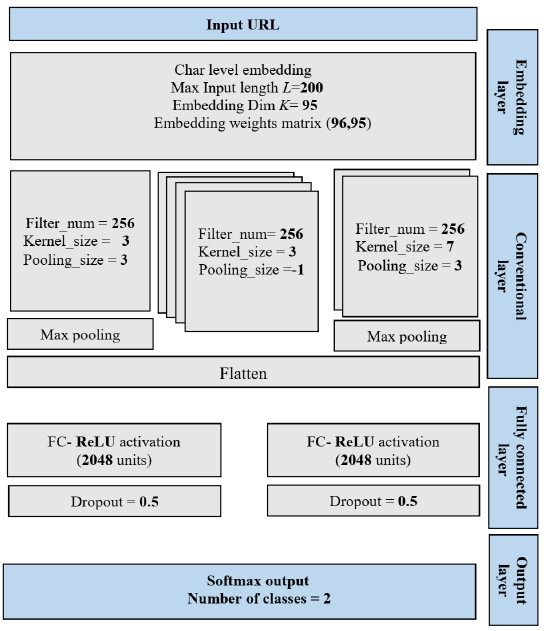
\includegraphics[width=0.8\linewidth]{report_img/cnn_configuration}
        \caption{CNN on character level embedding architecture~\cite{CharacterLevelCNN}}
        \label{fig:CNN}
    \end{figure}

    We implement the model with Keras, in the exact same setup as the models based on feature vectors.

    \begin{lstlisting}[language=Python, caption=CNN on character level embedding]
model = keras.Sequential(
    [
        layers.Input((150, 1)),
        layers.Convolution1D(
            kernel_size=3,
            filters=256,
            activation="relu",
        ),
        layers.MaxPooling1D(pool_size=3),
        layers.Convolution1D(kernel_size=3, filters=256, activation="relu"),
        layers.Convolution1D(kernel_size=3, filters=256, activation="relu"),
        layers.Convolution1D(kernel_size=3, filters=256, activation="relu"),
        layers.Convolution1D(kernel_size=3, filters=256, activation="relu"),
        layers.Convolution1D(kernel_size=7, filters=256, activation="relu"),
        layers.Convolution1D(kernel_size=7, filters=256, activation="relu"),
        layers.MaxPooling1D(pool_size=3),
        layers.Flatten(),
        layers.Dense(2048, activation="relu"),
        layers.Dropout(0.5),
        layers.Dense(2048, activation="relu"),
        layers.Dropout(0.5),
        layers.Dense(2, activation='softmax')
    ]
)
    \end{lstlisting}

    \subsubsection{Results}

    After 30 epochs, we achieve an accuracy of 97.61\% against 98.58\% for the original study\cite{CharacterLevelCNN} on the same dataset.
    \begin{figure}[H]
        \centering
        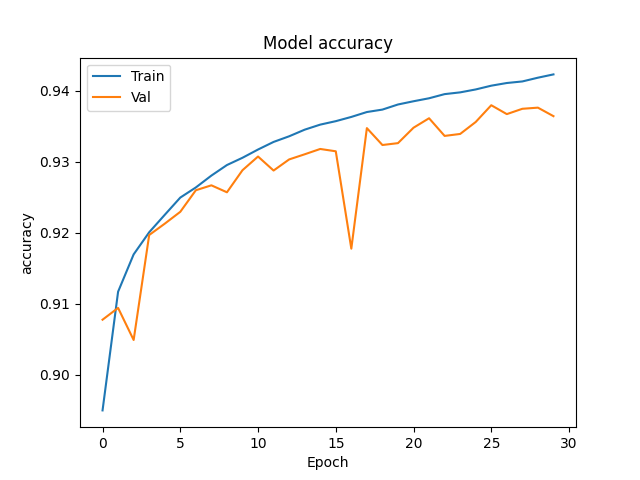
\includegraphics[width=0.8\textwidth]{report_img/nn_results/feature_vector_cnn_26/metric_accuracy}
        \caption{CNN accuracy}
        \label{fig:}
    \end{figure}

    On all metrics, we obtain:
    \begin{table}[H]
        \centering
        \begin{tabular}{|l|l|l|l|l|l|}
            \hline
            \textbf{Metric} & \textbf{Accuracy} & \textbf{F1 Score} & \textbf{Loss} & \textbf{Precision} & \textbf{Recall} \\ \hline
            \textbf{Value}  & 0.9762            & 0.9769            & 0.0831        & 0.9762             & 0.9762          \\ \hline
        \end{tabular}
        \caption{Validation Metrics}
        \label{tab:validation_metrics}
    \end{table}

    The evolution of further metrics can be found in\ref{sec:appendixC}.

    CNN model on character level is the model we reach the best accuracy among all the neural networks.
    Compared with the CNN on feature vector, we obtain a rise of +4\% accuracy.
    In return, the size of the model in memory as well as the training time increased significantly (x10 for training time).

    The difference with the original model of the study can be explained by the training time, as well as a different choice in the test set that has been chosen for computing the metrics.

    The study\cite{PhishingLoginURLDetection} also proposes a CNN at Character level that reaches 96.43\% accuracy on PIU 60k dataset.
    The smaller accuracy can be explained by the smaller size of their dataset (60k URL against 150k).

    \subsection{Large language model fine tuning}\label{subsec:large-language-model-finetuning}

    \subsubsection{Motivation of this implementation}

    Considering the recent success of large language models in Natural Language Processing (NLP) tasks, we decided to explore the potential of this approach for phishing URL detection.
    The objective is to leverage the pre-trained language model's knowledge of the English language, such as phishing terminology and common misspellings, to achieve a high accuracy.
    We expect this approach to be more efficient than the character-level embedding because it is able to learn the spelling of words and the context in which they are used.
    Besides having a personal interest in LLM, only a few studies have been done on this approach, so we found it interesting to propose our new approach and modeling.

    \subsubsection{Implementation}

    The Python package \texttt{transformers} from HuggingFace provides many pre-trained language models that can be directly applied on a task or fine-tuned on a specific dataset.
    We chose to use Bert because it is the most popular language model and it has been shown to be effective on many NLP task.
    HuggingFace provides a multilingual version of Bert since our dataset contains URLs in different languages.

    First, we tokenize our dataset into Bert embeddings using the \texttt{transformer} library's provided \texttt{BertTokenizer}.
    Note that for this task, we use a subsample of $100.000$ URLs from our dataset, since we are limited in computing power.

    \begin{lstlisting}[language=Python, caption=Tokenizing using Bert]
tokenizer = BertTokenizer.from_pretrained('bert-base-multilingual-uncased')

def encode(x): # simplified definition of encode
    return tokenizer.encode(x)

input_ids_train, attention_masks_train = encode(train_x)
input_ids_val, attention_masks_val = encode(val_x)
input_ids_test, attention_masks_test = encode(test_x)
    \end{lstlisting}

    We then used the \texttt{TFBertForSequenceClassification} class to train the model on our dataset.
    This model is a Bert model with a classification layer on top of it (i.e. dropout and dense layer).
    The entire model is fine-tuned on our dataset.
    The authors of~\cite{devlin2018bert} suggest 2,3, or 4 epochs with a batch size of around 16 and learning rates in the order of e-5.
    For this task, we use a batch size of 6 and a learning rate of 1e-5 to reduce the GPU memory usage.

    \begin{lstlisting}[language=Python, caption=Fine tuning Bert]
model = TFBertForSequenceClassification.from_pretrained('bert-base-multilingual-uncased')
model.compile(optimizer=tf.keras.optimizers.Adam(learning_rate=1e-5), loss=tf.keras.losses.SparseCategoricalCrossentropy(from_logits=True), metrics="accuracy")

model.fit(
    [input_ids_train, attention_masks_train],
    labels_train,
    validation_data=([input_ids_val, attention_masks_val], labels_val),
    batch_size=6,
    epochs=3
)
    \end{lstlisting}

    \subsubsection{Results}

    After 4 epochs, we achieve an accuracy of 99.15\%, the best accuracy among all the models we have trained.
    \cite{PhishBert} also uses LLM: They pre-train a model on 3 billion URL before fine tuning it for phishing classification.
    If they do not report the concrete accuracy outside their figures, we can deduce from their graphs that we have a similar accuracy to their model, without going through a similar pre-training phase.

    \begin{figure}[H]
        \centering
        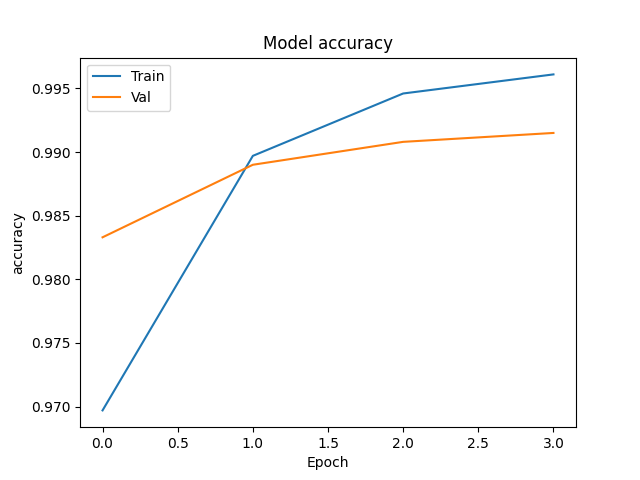
\includegraphics[width=0.8\textwidth]{report_img/bert_results/metric_accuracy}
        \caption{Bert accuracy}
        \label{fig:}
    \end{figure}

    We may have been able to get a higher accuracy by fine-tuning the learning rate and running the training for longer, but we are limited in computing power.
    Perhaps using the complete dataset would also considerably improve the accuracy, considering that ~\cite{PhishBert} notes that from 10\% to 80\%, their accuracy increased several percentile points.

    \section{Conclusion}\label{sec:conclusion}

    Our study compares a range of machine learning algorithms, including Large Language Models (LLMs), on a consistent dataset.
    We critically assessed the practicality of each of our model together with examples of the literature.
    For feature extraction, we focused on the ease of feature construction and the need for external data sources like website queries or third-party information.
    For models relying on feature vectors, our findings reveal that statistical models can achieve performance on par with neural networks.
    Such models based on feature vectors are particularly valuable for their explain-ability, aiding in understanding the nature of URLs in phishing detection.
    This understanding of the decision criteria could further guide the development of security systems.
    However, in terms of accuracy, methods that rely on string embeddings, typically found in neural networks, have an edge.
    Crucially, the ability to continually update the model architecture is essential, allowing it to adapt to evolving phishing tactics.
    Pretrained LLMs show promise due to their ease of training and remarkable performance.
    Though large neural networks may be impractical for running locally in browsers, they can be used in existing services such as Google SafeBrowsing.
    In addition, the recent popularity influx of LLMs has led to browser extensions that utilize LLMs for common browsing tasks.
    This pushes LLM to be the most practical solution for browser developers.

    Considering the remarkably high accuracy of our models and the models provided in the literature, we believe that the next step is to research how to integrate these models into the browsers.
    A pivotal question is how to adapt these algorithms to keep pace with evolving phishing trends while maintaining their accuracy, presenting a continuous challenge of continuous web crawling for new malicious URLs.
    Besides the evolution of phishing URLs, the trend of URL shortening services, which obscure real phishing URLs, renders these models ineffective, which has not been addressed yet.
    Additionally, investigating adversarial attacks is critical to bolster the robustness of these models.

    To advance the field in these directions, it is imperative that studies publish their datasets and clear implementation details, enabling reproducibility for industry integration.

    \bibliographystyle{plain}
    \bibliography{refs}

    \appendix


    \section{Appendix A: k search graphs}\label{sec:appendixA}

    \begin{figure}[H]
        \centering
        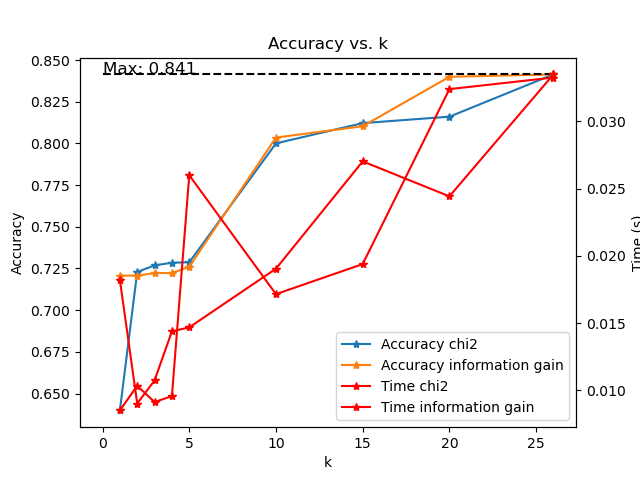
\includegraphics[width=0.8\textwidth]{report_img/k_search/linear_svc}
        \caption{Linear SVC accuracy depending on the k number of chosen features}
        \label{fig:}
    \end{figure}

    \begin{figure}[H]
        \centering
        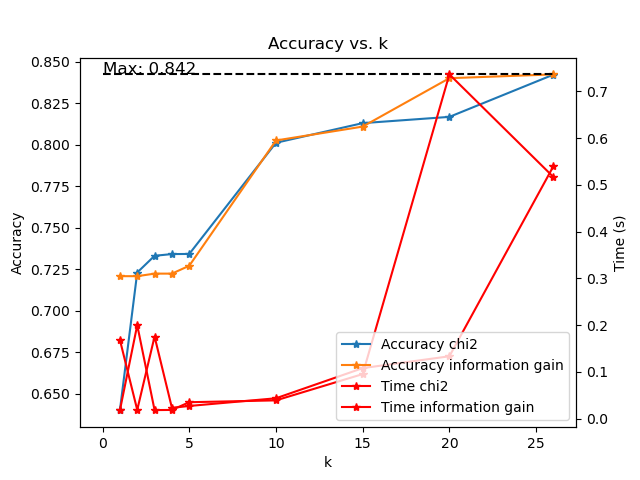
\includegraphics[width=0.8\textwidth]{report_img/k_search/logistic_regression}
        \caption{Logistic regression accuracy depending on the k number of chosen features}
        \label{fig:}
    \end{figure}

    \begin{figure}[H]
        \centering
        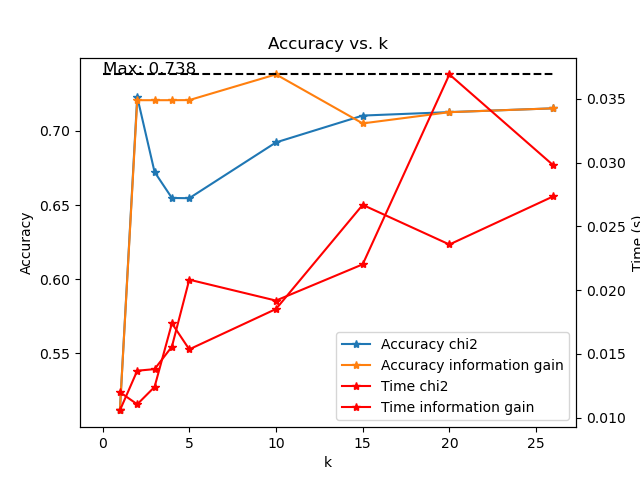
\includegraphics[width=0.8\textwidth]{report_img/k_search/naive_bayes}
        \caption{Naive Bayes accuracy depending on the k number of chosen features}
        \label{fig:}
    \end{figure}

    \begin{figure}[H]
        \centering
        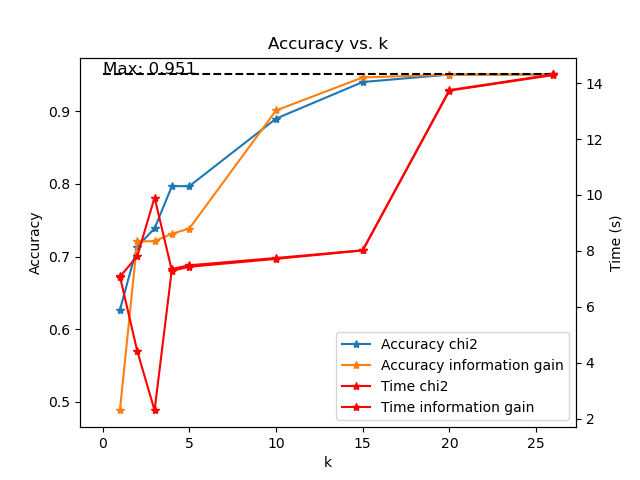
\includegraphics[width=0.8\textwidth]{report_img/k_search/nearest_neighbors}
        \caption{Nearest Neighbours accuracy depending on the k number of chosen features}
        \label{fig:}
    \end{figure}

    \begin{figure}[H]
        \centering
        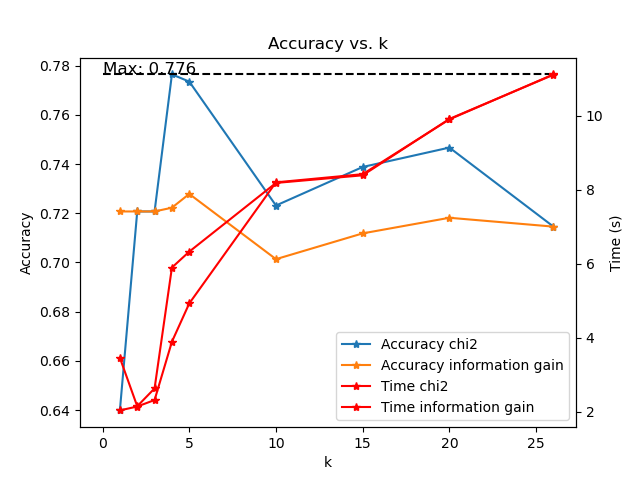
\includegraphics[width=0.8\textwidth]{report_img/k_search/random_forest}
        \caption{Random Forest accuracy depending on the k number of chosen features}
        \label{fig:}
    \end{figure}


    \section{Appendix B: param search}\label{sec:appendixB}

    \begin{figure}[H]
        \centering
        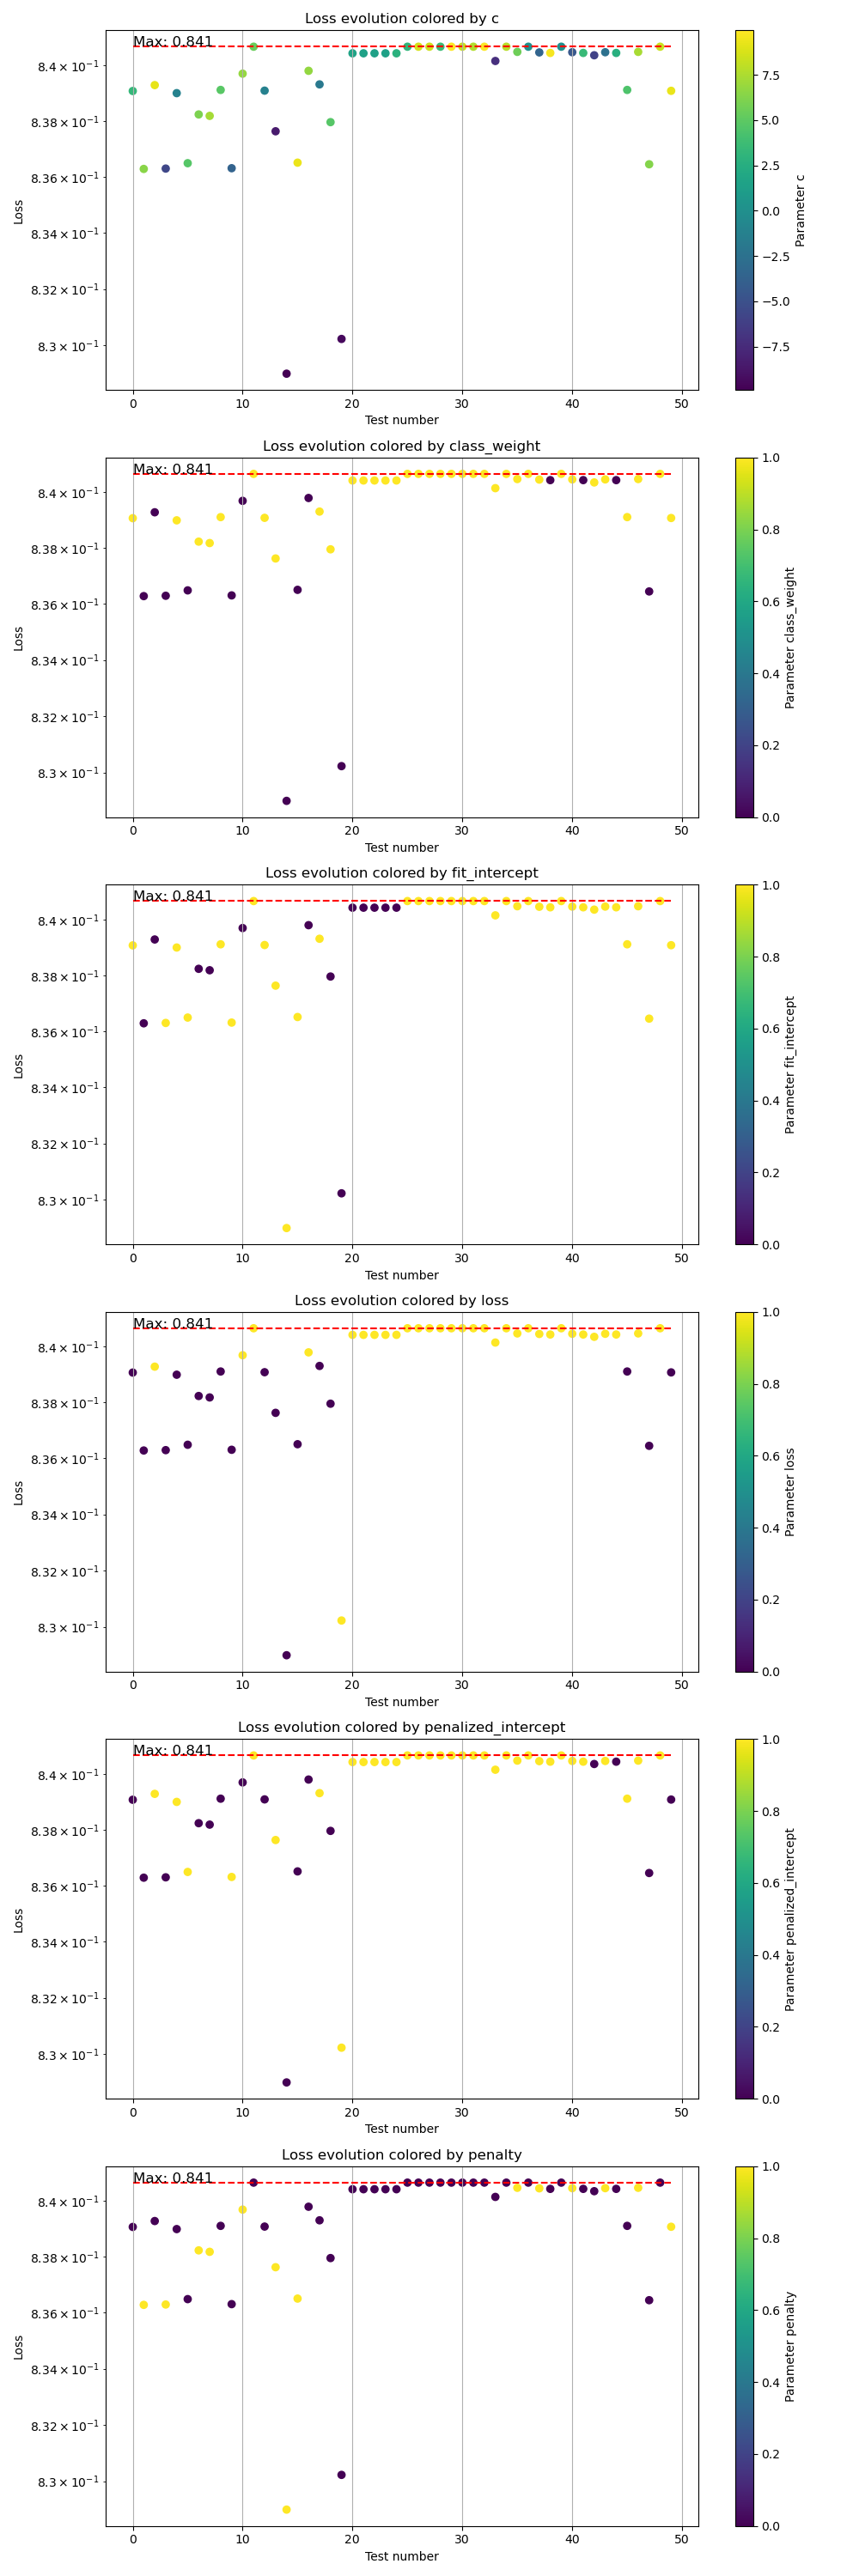
\includegraphics[width=0.5\textwidth]{report_img/param_search/linear_svc}
        \caption{Parameter search for linear SVC}
        \label{fig:}
    \end{figure}

    \begin{figure}[H]
        \centering
        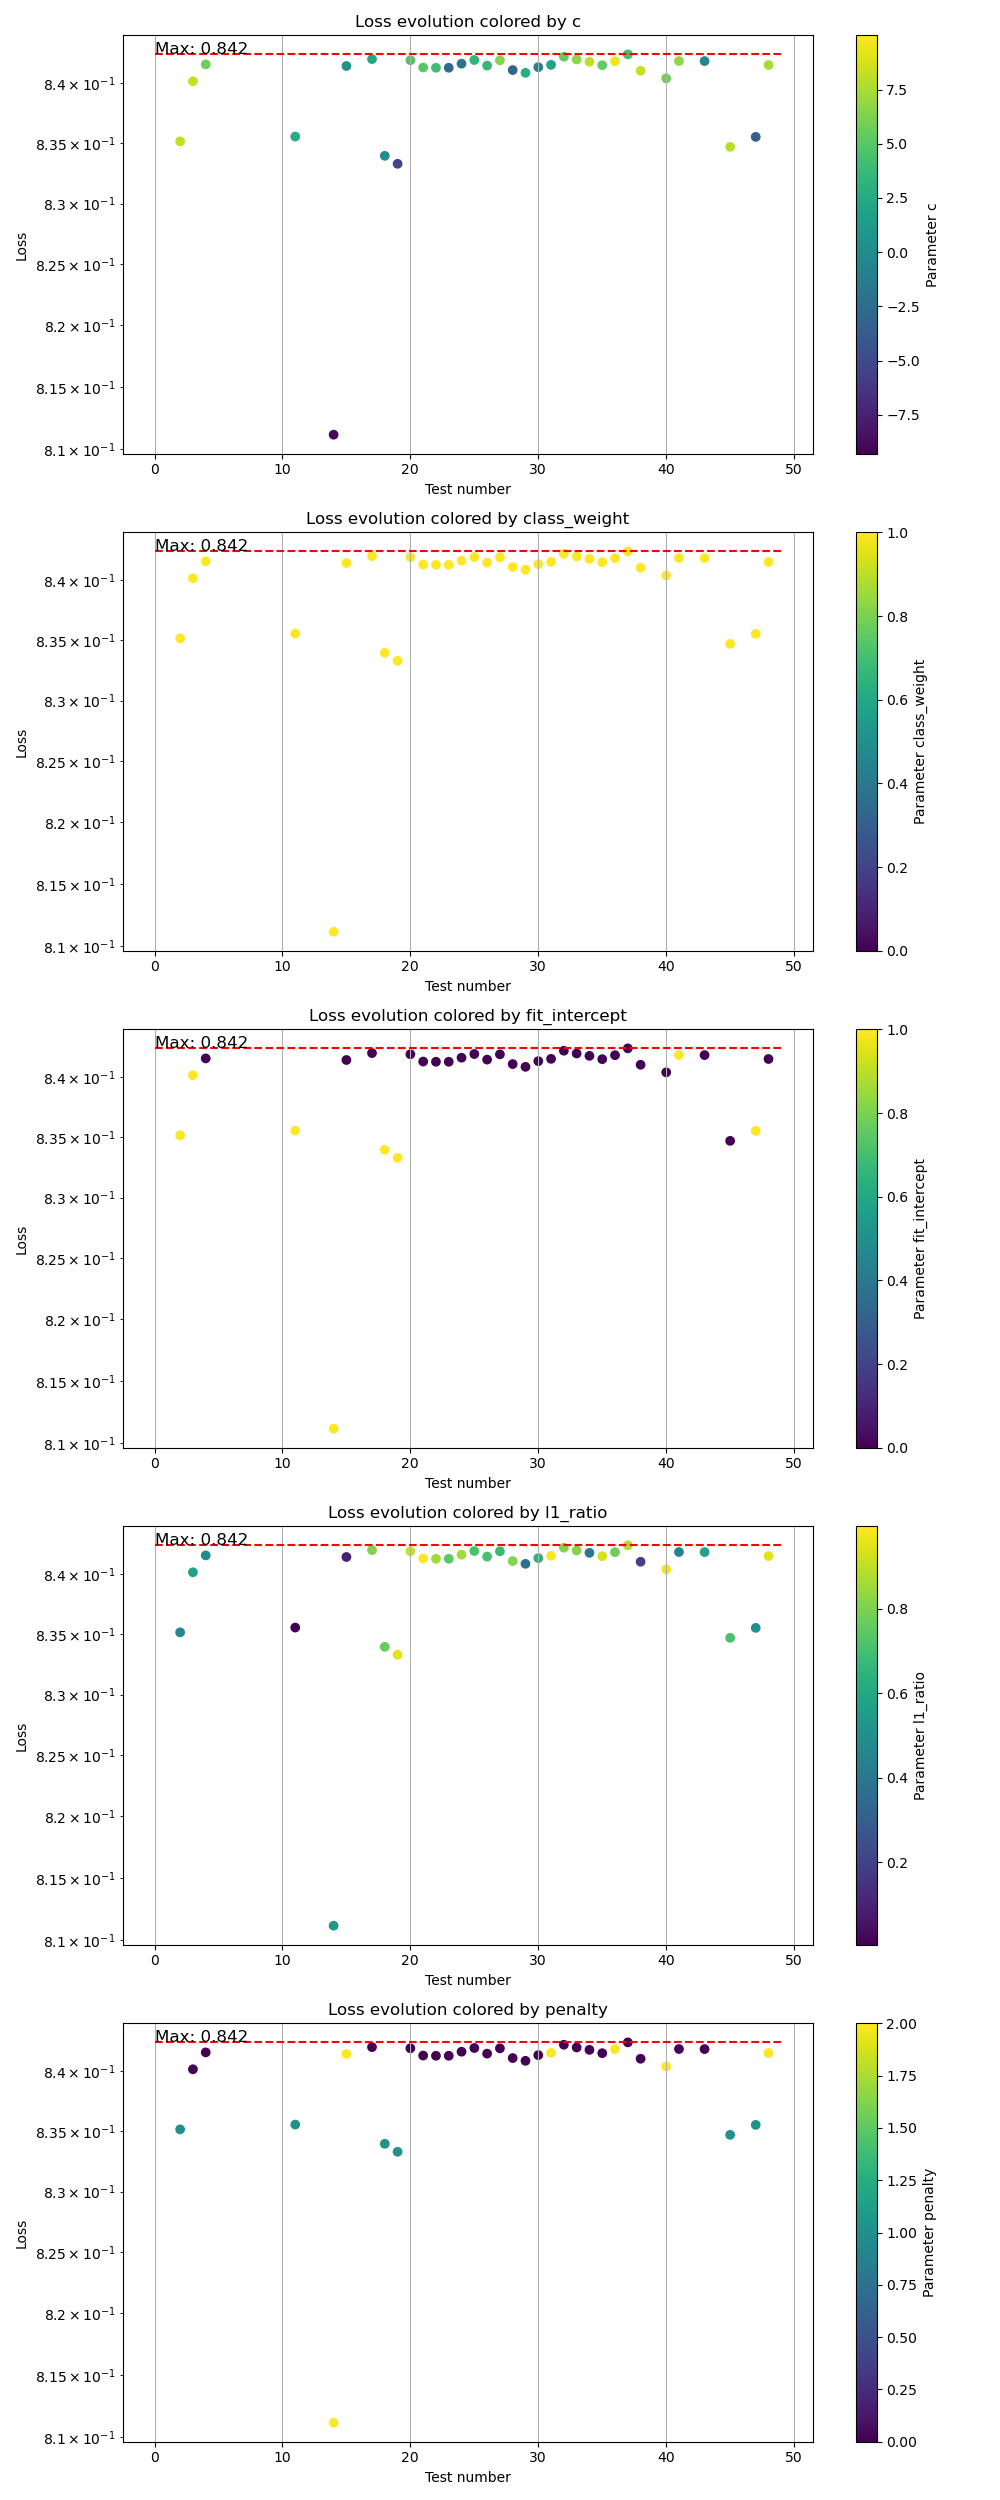
\includegraphics[width=0.5\textwidth]{report_img/param_search/logistic_regression}
        \caption{Parameter search for logistic regression}
        \label{fig:}
    \end{figure}

    \begin{figure}[H]
        \centering
        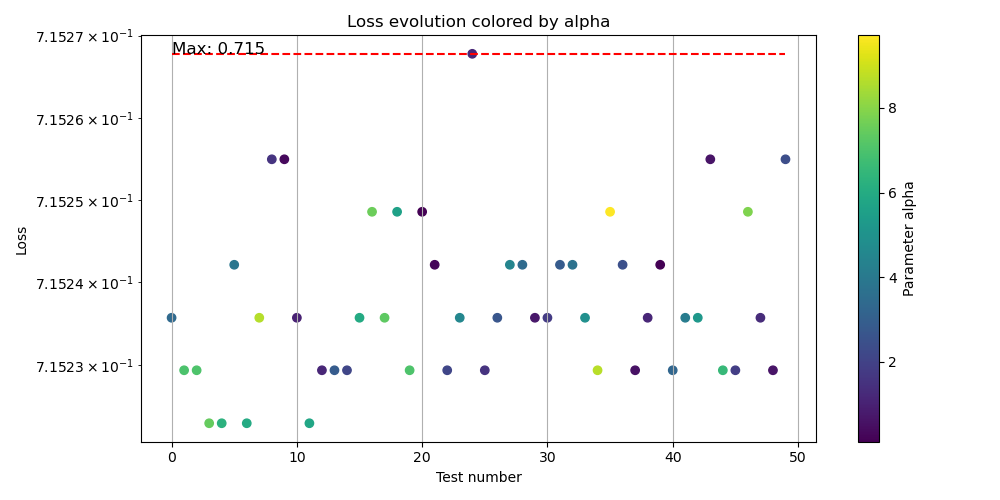
\includegraphics[width=0.5\textwidth]{report_img/param_search/naive_bayes}
        \caption{Parameter search for Naive Bayes}
        \label{fig:}
    \end{figure}

    \begin{figure}
        \centering
        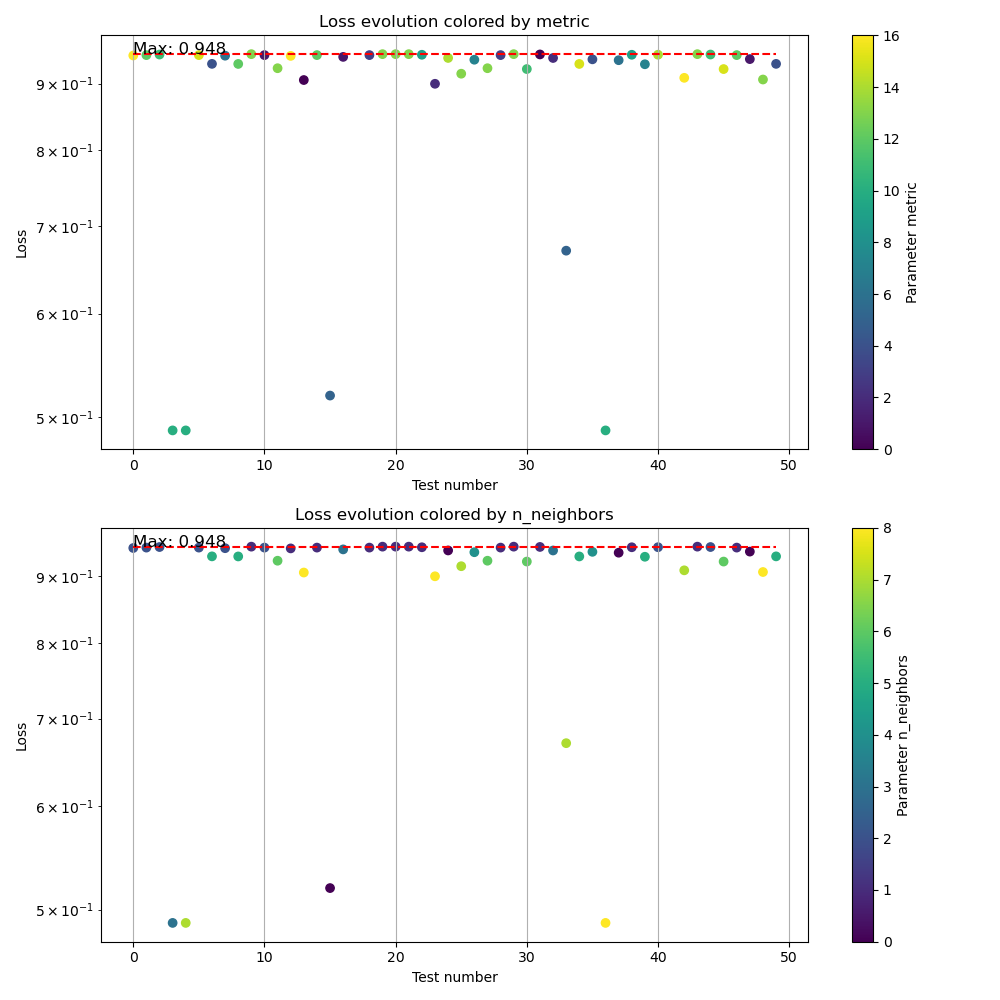
\includegraphics[width=0.5\textwidth]{report_img/param_search/nearest_neighbors}
        \caption{Parameter search for Nearest Neighbours}
        \label{fig:}
    \end{figure}

    \begin{figure}[H]
        \centering
        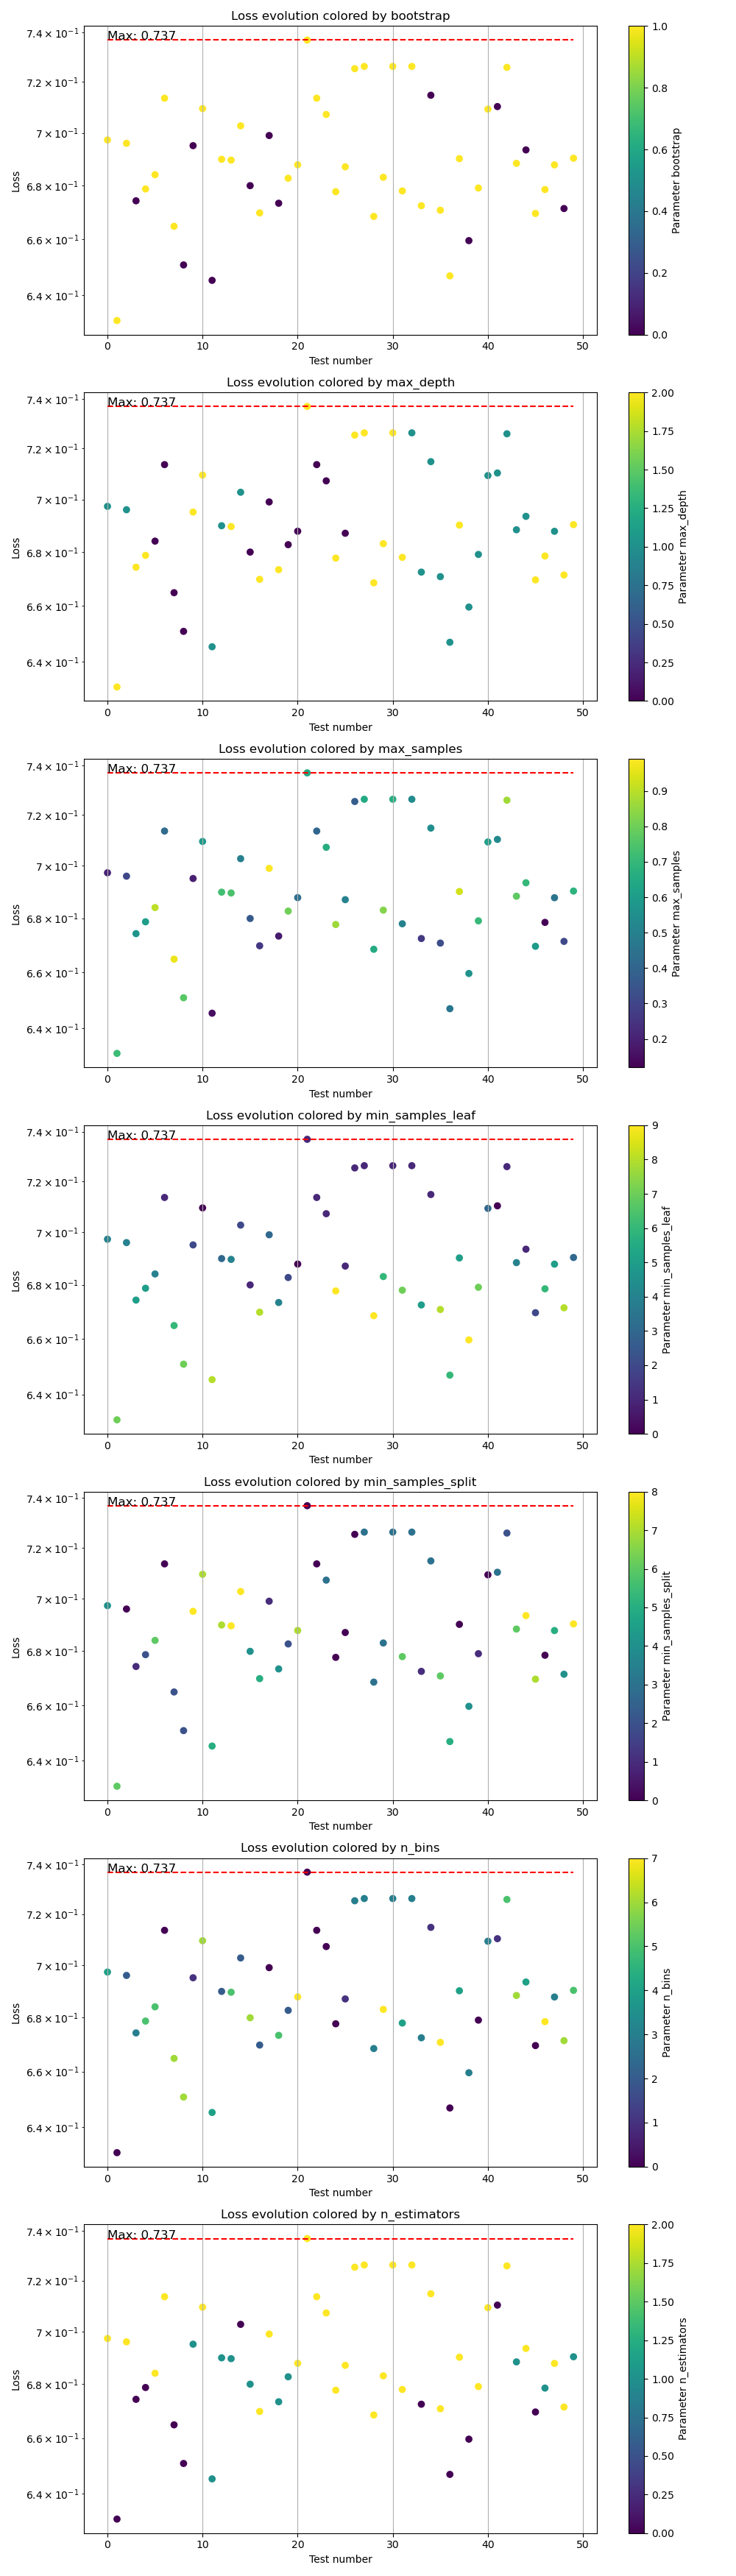
\includegraphics[width=0.5\textwidth]{report_img/param_search/random_forest}
        \caption{Parameter search for random forest}
        \label{fig:}
    \end{figure}


    \section{Appendix C: neural network results}\label{sec:appendixC}

    \subsection{Feature Based CNN}

    \begin{figure}[H]
        \centering
        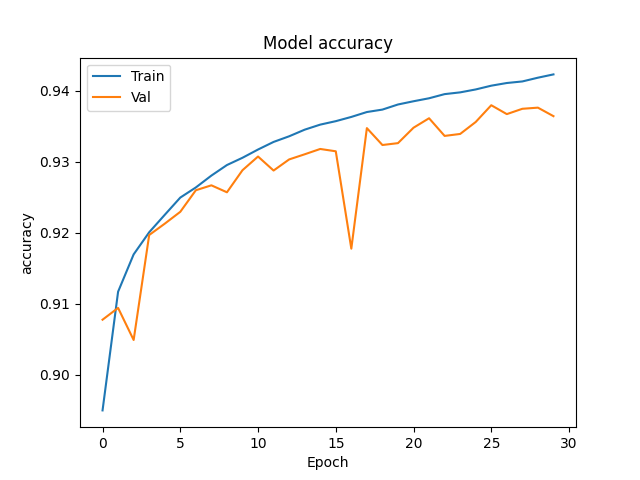
\includegraphics[width=0.8\textwidth]{report_img/nn_results/feature_vector_cnn_26/metric_accuracy}
        \caption{CNN accuracy}
        \label{fig:}
    \end{figure}

    \begin{figure}[H]
        \centering
        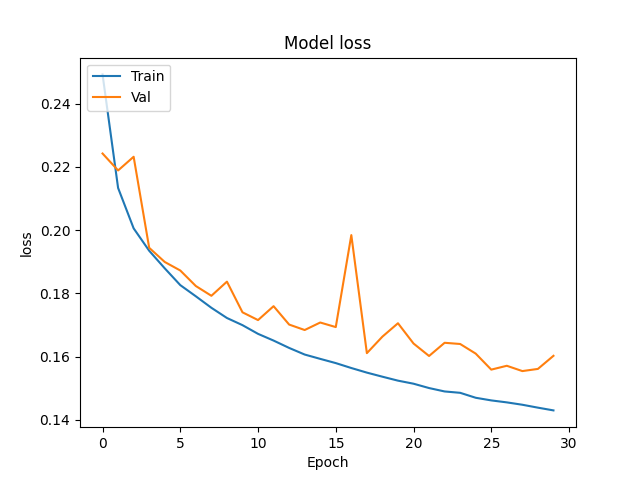
\includegraphics[width=0.8\textwidth]{report_img/nn_results/feature_vector_cnn_26/metric_loss}
        \caption{CNN loss}
        \label{fig:}
    \end{figure}

    \begin{figure}[H]
        \centering
        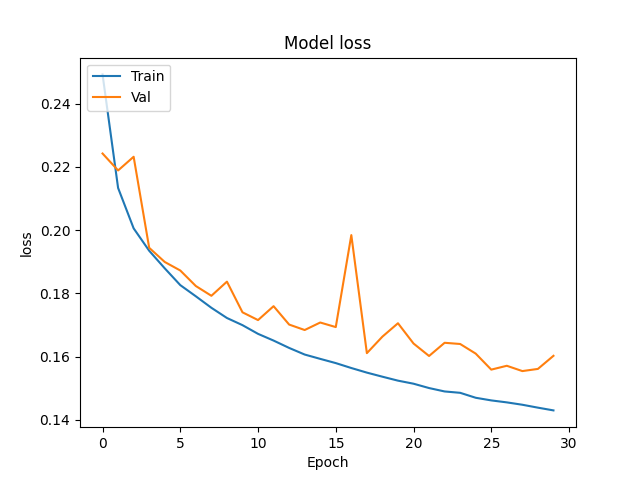
\includegraphics[width=0.8\textwidth]{report_img/nn_results/feature_vector_cnn_26/metric_loss}
        \caption{CNN loss}
        \label{fig:}
    \end{figure}

    \begin{figure}[H]
        \centering
        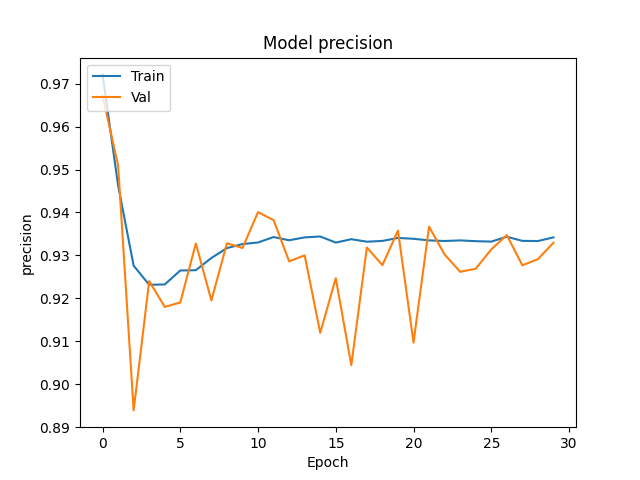
\includegraphics[width=0.8\textwidth]{report_img/nn_results/feature_vector_cnn_26/metric_precision}
        \caption{CNN precision}
        \label{fig:}
    \end{figure}

    \subsection{Feature Based DNN}

    \begin{figure}[H]
        \centering
        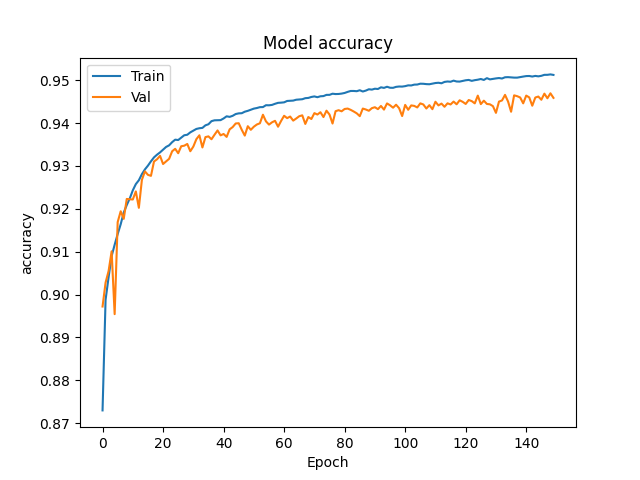
\includegraphics[width=0.8\textwidth]{report_img/nn_results/feature_vector_dnn_26/metric_150_accuracy}
        \caption{DNN accuracy}
        \label{fig:}
    \end{figure}

    \begin{figure}[H]
        \centering
        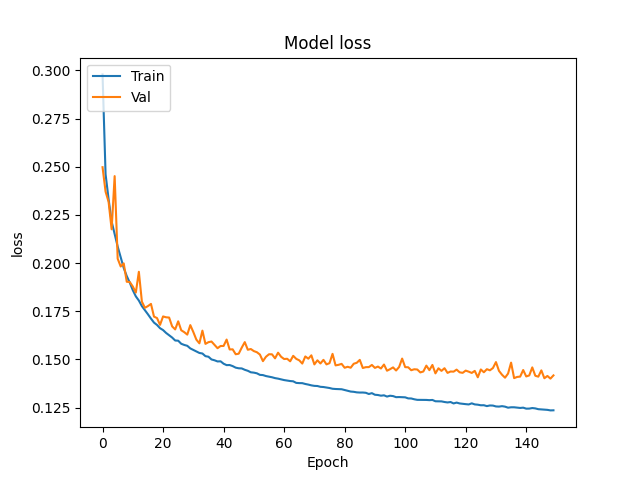
\includegraphics[width=0.8\textwidth]{report_img/nn_results/feature_vector_dnn_26/metric_150_loss}
        \caption{DNN loss}
        \label{fig:}
    \end{figure}

    \begin{figure}[H]
        \centering
        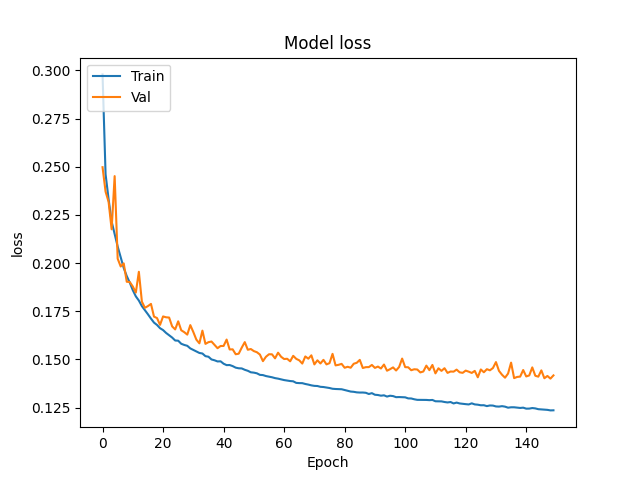
\includegraphics[width=0.8\textwidth]{report_img/nn_results/feature_vector_dnn_26/metric_150_loss}
        \caption{DNN loss}
        \label{fig:}
    \end{figure}

    \begin{figure}[H]
        \centering
        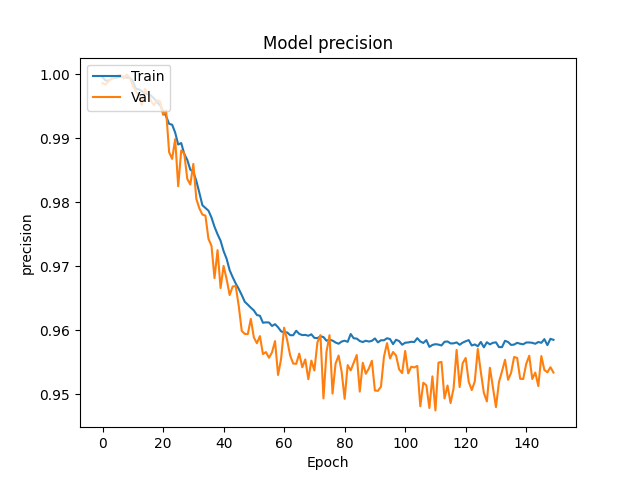
\includegraphics[width=0.8\textwidth]{report_img/nn_results/feature_vector_dnn_26/metric_150_precision}
        \caption{DNN precision}
        \label{fig:}
    \end{figure}

    \subsection{Feature Based LSTM}

    \begin{figure}[H]
        \centering
        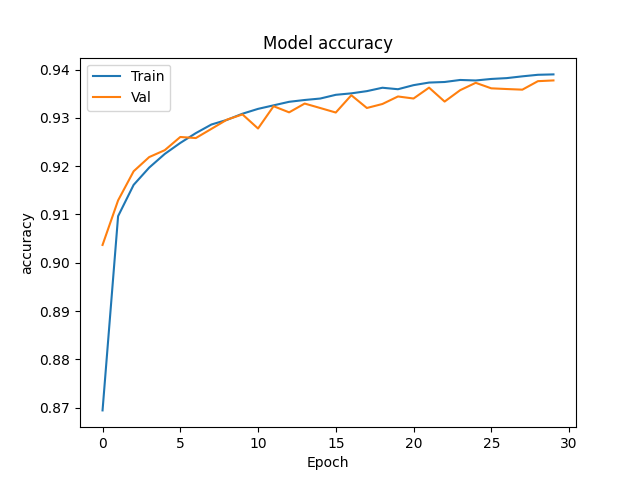
\includegraphics[width=0.8\textwidth]{report_img/nn_results/feature_vector_lstm_26/metric_accuracy}
        \caption{LSTM accuracy}
        \label{fig:}
    \end{figure}

    \begin{figure}[H]
        \centering
        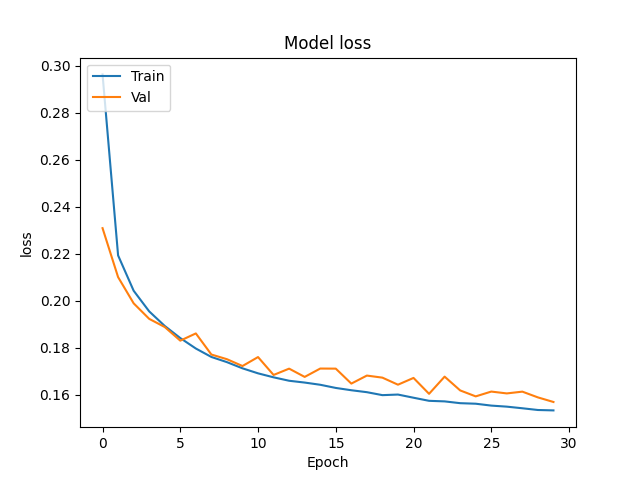
\includegraphics[width=0.8\textwidth]{report_img/nn_results/feature_vector_lstm_26/metric_loss}
        \caption{LSTM loss}
        \label{fig:}
    \end{figure}

    \begin{figure}[H]
        \centering
        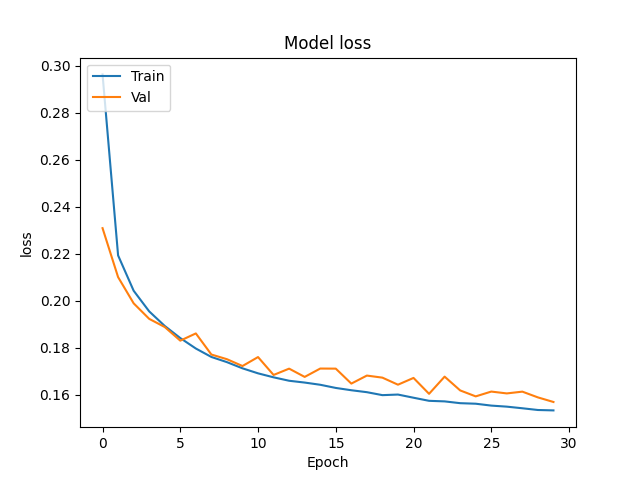
\includegraphics[width=0.8\textwidth]{report_img/nn_results/feature_vector_lstm_26/metric_loss}
        \caption{LSTM loss}
        \label{fig:}
    \end{figure}

    \begin{figure}[H]
        \centering
        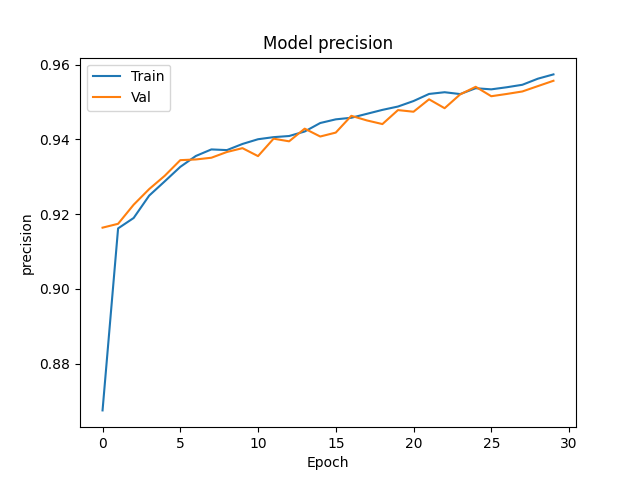
\includegraphics[width=0.8\textwidth]{report_img/nn_results/feature_vector_lstm_26/metric_precision}
        \caption{LSTM precision}
        \label{fig:}
    \end{figure}

    \subsection{String Embedding Based CNN}

    \begin{figure}[H]
        \centering
        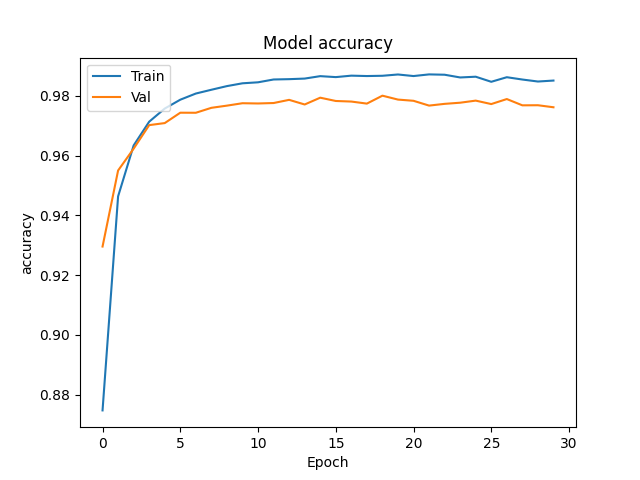
\includegraphics[width=0.8\textwidth]{report_img/nn_results/string_embedding_cnn_26/metric_accuracy}
        \caption{CNN accuracy}
        \label{fig:}
    \end{figure}

    \begin{figure}[H]
        \centering
        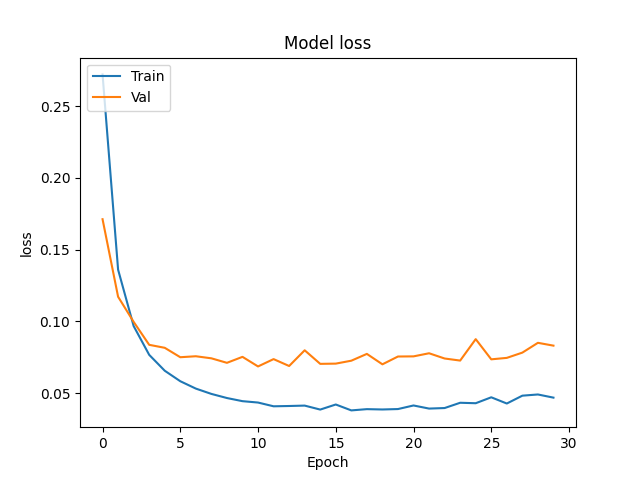
\includegraphics[width=0.8\textwidth]{report_img/nn_results/string_embedding_cnn_26/metric_loss}
        \caption{CNN loss}
        \label{fig:}
    \end{figure}

    \begin{figure}[H]
        \centering
        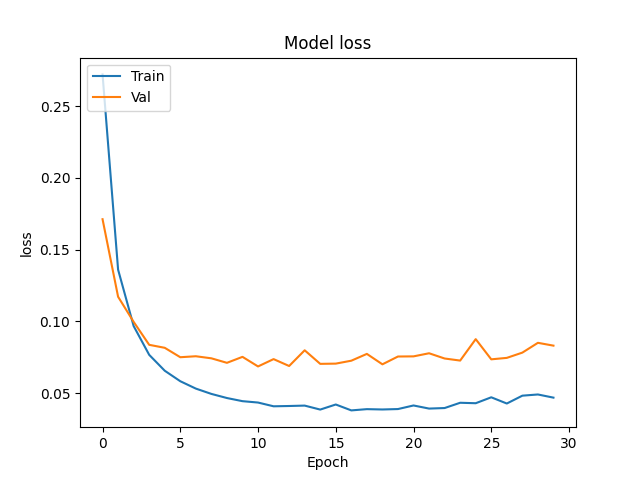
\includegraphics[width=0.8\textwidth]{report_img/nn_results/string_embedding_cnn_26/metric_loss}
        \caption{CNN loss}
        \label{fig:}
    \end{figure}

    \begin{figure}[H]
        \centering
        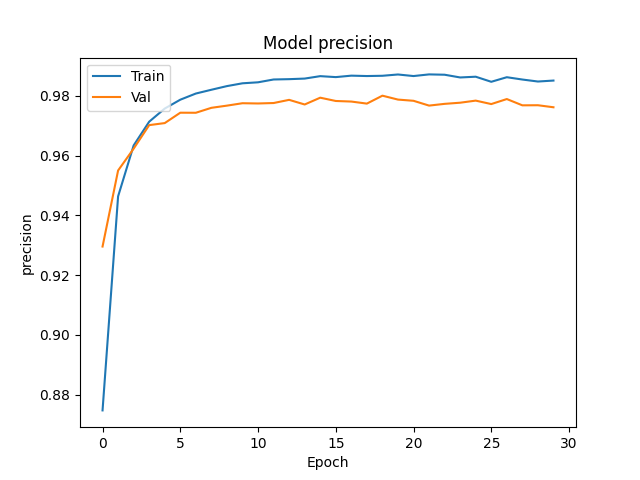
\includegraphics[width=0.8\textwidth]{report_img/nn_results/string_embedding_cnn_26/metric_precision}
        \caption{CNN precision}
        \label{fig:}
    \end{figure}
\end{document}